\documentclass[10pt,a4paper]{article}
\usepackage[utf8]{inputenc}
\usepackage[T1]{fontenc}
\usepackage{lmodern}
\usepackage[margin=1in]{geometry}
\usepackage{amsmath,amssymb,amsthm}
\usepackage{booktabs}
\usepackage{graphicx}
\usepackage{microtype}
\usepackage[numbers,sort&compress]{natbib}
\usepackage{xcolor}
\usepackage[colorlinks=true,linkcolor=blue!50!black,citecolor=blue!50!black,urlcolor=blue!50!black]{hyperref}
\usepackage{enumitem}
\usepackage{array}
\usepackage{caption}
\captionsetup{font=small,labelfont=bf}

\IfFileExists{numbers.tex}{% generated by experiments/make_numbers.py -- do not edit
\newcommand{\MetaSeed}{20260930}
\newcommand{\MetaPython}{3.11.15}
\newcommand{\MetaNumpy}{2.4.6}
\newcommand{\MetaScipy}{1.17.1}
\newcommand{\MetaSeconds}{52}
\newcommand{\MetaCpuSeconds}{53}
\newcommand{\MetaSecondsTotal}{56}
\newcommand{\MetaCpuSecondsTotal}{57}
\newcommand{\MetaScriptSha}{5b309162009c}
\newcommand{\MetaDate}{2026-10-03}
\newcommand{\EzeroCDthird}{\ensuremath{1.7\times 10^{-10}}}
\newcommand{\EzeroCESthird}{\ensuremath{5.7\times 10^{-10}}}
\newcommand{\EoneN}{2000}
\newcommand{\EoneReps}{20}
\newcommand{\EoneXbarK}{2.0}
\newcommand{\EoneXbarL}{1.0}
\newcommand{\EoneCorr}{0.5}
\newcommand{\EoneSlopeOneCDLN}{2.00}
\newcommand{\EoneSlopeTwoCDLN}{3.12}
\newcommand{\EoneSlopeThreeCDLN}{4.01}
\newcommand{\EoneSlopeOneSeCDLN}{0.00}
\newcommand{\EoneSlopeTwoSeCDLN}{0.26}
\newcommand{\EoneSlopeThreeSeCDLN}{0.00}
\newcommand{\EoneCiHalfRelMaxCDLN}{70}
\newcommand{\EoneConeLargestCDLN}{0.42}
\newcommand{\EoneConeWholeCDLN}{no}
\newcommand{\EoneConeFirstFailCDLN}{0.56}
\newcommand{\EoneSigmaMaxCDLN}{1.0}
\newcommand{\EoneRtoAtMaxCDLN}{0.31}
\newcommand{\EoneRttCellsCDLN}{15}
\newcommand{\EoneCellsCDLN}{17}
\newcommand{\EoneRttMinCDLN}{0.002}
\newcommand{\EoneRatioGtOneSigmaCDLN}{0.75}
\newcommand{\EoneCertSigmaCDLN}{0.056}
\newcommand{\EoneCertBoxSigmaCDLN}{0.042}
\newcommand{\EoneCertConeSigmaCDLN}{0.018}
\newcommand{\EoneCertConeBoxSigmaCDLN}{0.018}
\newcommand{\EoneBoundSigmaNonobsCDLN}{0.10}
\newcommand{\EoneEtwoOverBtwoMaxCDLN}{0.018}
\newcommand{\EoneBoxOverSegCDLN}{7215}
\newcommand{\EoneBoundHoldsCDLN}{yes}
\newcommand{\EoneSlopeOneCDSU}{2.00}
\newcommand{\EoneSlopeTwoCDSU}{4.00}
\newcommand{\EoneSlopeThreeCDSU}{4.00}
\newcommand{\EoneSlopeOneSeCDSU}{0.00}
\newcommand{\EoneSlopeTwoSeCDSU}{0.00}
\newcommand{\EoneSlopeThreeSeCDSU}{0.00}
\newcommand{\EoneCiHalfRelMaxCDSU}{3}
\newcommand{\EoneConeLargestCDSU}{0.50}
\newcommand{\EoneConeWholeCDSU}{yes}
\newcommand{\EoneConeFirstFailCDSU}{--}
\newcommand{\EoneSigmaMaxCDSU}{0.5}
\newcommand{\EoneRtoAtMaxCDSU}{5.87}
\newcommand{\EoneRttCellsCDSU}{0}
\newcommand{\EoneCellsCDSU}{15}
\newcommand{\EoneRttMinCDSU}{1.000}
\newcommand{\EoneRatioGtOneSigmaCDSU}{0.50}
\newcommand{\EoneCertSigmaCDSU}{0.071}
\newcommand{\EoneCertBoxSigmaCDSU}{0.053}
\newcommand{\EoneCertConeSigmaCDSU}{0.023}
\newcommand{\EoneCertConeBoxSigmaCDSU}{0.023}
\newcommand{\EoneBoundSigmaNonobsCDSU}{0.12}
\newcommand{\EoneEtwoOverBtwoMaxCDSU}{0.016}
\newcommand{\EoneBoxOverSegCDSU}{13}
\newcommand{\EoneBoundHoldsCDSU}{yes}
\newcommand{\EoneSlopeOneCESLN}{2.00}
\newcommand{\EoneSlopeTwoCESLN}{3.18}
\newcommand{\EoneSlopeThreeCESLN}{4.00}
\newcommand{\EoneSlopeOneSeCESLN}{0.00}
\newcommand{\EoneSlopeTwoSeCESLN}{0.24}
\newcommand{\EoneSlopeThreeSeCESLN}{0.00}
\newcommand{\EoneCiHalfRelMaxCESLN}{52}
\newcommand{\EoneConeLargestCESLN}{0.42}
\newcommand{\EoneConeWholeCESLN}{no}
\newcommand{\EoneConeFirstFailCESLN}{0.56}
\newcommand{\EoneSigmaMaxCESLN}{1.0}
\newcommand{\EoneRtoAtMaxCESLN}{0.48}
\newcommand{\EoneRttCellsCESLN}{13}
\newcommand{\EoneCellsCESLN}{17}
\newcommand{\EoneRttMinCESLN}{0.035}
\newcommand{\EoneRatioGtOneSigmaCESLN}{0.75}
\newcommand{\EoneSlopeOneCESSU}{2.00}
\newcommand{\EoneSlopeTwoCESSU}{4.00}
\newcommand{\EoneSlopeThreeCESSU}{4.00}
\newcommand{\EoneSlopeOneSeCESSU}{0.00}
\newcommand{\EoneSlopeTwoSeCESSU}{0.00}
\newcommand{\EoneSlopeThreeSeCESSU}{0.00}
\newcommand{\EoneCiHalfRelMaxCESSU}{2}
\newcommand{\EoneConeLargestCESSU}{0.50}
\newcommand{\EoneConeWholeCESSU}{yes}
\newcommand{\EoneConeFirstFailCESSU}{--}
\newcommand{\EoneSigmaMaxCESSU}{0.5}
\newcommand{\EoneRtoAtMaxCESSU}{5.64}
\newcommand{\EoneRttCellsCESSU}{0}
\newcommand{\EoneCellsCESSU}{15}
\newcommand{\EoneRttMinCESSU}{1.000}
\newcommand{\EoneRatioGtOneSigmaCESSU}{0.50}
\newcommand{\EoneLooseMin}{56}
\newcommand{\EoneLooseMax}{1064}
\newcommand{\EonebN}{2000}
\newcommand{\EonebReps}{20}
\newcommand{\EonebSdTheta}{0.19}
\newcommand{\EonebSigmaCov}{0.18}
\newcommand{\EonebRatioSmallest}{\ensuremath{7\times 10^{3}}}
\newcommand{\EonebPredMin}{0.81}
\newcommand{\EonebPredMax}{0.92}
\newcommand{\EonecReps}{60}
\newcommand{\EonecSlopeTwoNSmall}{3.16}
\newcommand{\EonecSlopeTwoSeNSmall}{0.09}
\newcommand{\EonecSlopeThreeNSmall}{4.00}
\newcommand{\EonecSlopeThreeSeNSmall}{0.006}
\newcommand{\EonecThirdTermNSmall}{\ensuremath{8.0\times 10^{-9}}}
\newcommand{\EonecNSmall}{200}
\newcommand{\EonecSlopeTwoNMid}{3.50}
\newcommand{\EonecSlopeTwoSeNMid}{0.10}
\newcommand{\EonecSlopeThreeNMid}{4.00}
\newcommand{\EonecSlopeThreeSeNMid}{0.002}
\newcommand{\EonecThirdTermNMid}{\ensuremath{2.3\times 10^{-9}}}
\newcommand{\EonecNMid}{2000}
\newcommand{\EonecSlopeTwoNLarge}{4.05}
\newcommand{\EonecSlopeTwoSeNLarge}{0.10}
\newcommand{\EonecSlopeThreeNLarge}{4.00}
\newcommand{\EonecSlopeThreeSeNLarge}{0.001}
\newcommand{\EonecThirdTermNLarge}{\ensuremath{2.3\times 10^{-9}}}
\newcommand{\EonecNLarge}{20000}
\newcommand{\EonecSlopeTwoNHuge}{3.96}
\newcommand{\EonecSlopeTwoSeNHuge}{0.02}
\newcommand{\EonecSlopeThreeNHuge}{4.00}
\newcommand{\EonecSlopeThreeSeNHuge}{0.000}
\newcommand{\EonecThirdTermNHuge}{\ensuremath{2.6\times 10^{-9}}}
\newcommand{\EonecNHuge}{200000}
\newcommand{\EonecNs}{200, 2000, 20000, 200000}
\newcommand{\EonecSlopeThreeMin}{4.00}
\newcommand{\EonecSlopeThreeMax}{4.00}
\newcommand{\EonecSlopeThreeSeMax}{0.006}
\newcommand{\EtwoN}{2000}
\newcommand{\EtwoReps}{20}
\newcommand{\EtwoCells}{168}
\newcommand{\EtwoTwoSided}{all}
\newcommand{\EtwoLowerInformative}{33}
\newcommand{\EtwoCrossingCells}{107}
\newcommand{\EtwoIdentityGap}{\ensuremath{2\times 10^{-15}}}
\newcommand{\EtwoSlopeCappedLN}{1.01}
\newcommand{\EtwoSlopeSmoothLN}{3.52}
\newcommand{\EtwoSlopeCappedSU}{1.00}
\newcommand{\EtwoSlopeSmoothSU}{4.00}
\newcommand{\EtwoSlopeCappedSeLN}{0.003}
\newcommand{\EtwoSlopeSmoothSeLN}{0.21}
\newcommand{\EtwoSlopeTransitionSe}{0.11}
\newcommand{\EtwoRatioMin}{0.38}
\newcommand{\EtwoRatioMax}{1.40}
\newcommand{\EtwoAmplification}{\ensuremath{1\times 10^{6}}}
\newcommand{\EtwoEtwoCapped}{\ensuremath{2.8\times 10^{-3}}}
\newcommand{\EtwoEtwoSmooth}{\ensuremath{2.4\times 10^{-9}}}
\newcommand{\EtwoEtwoCappedLo}{\ensuremath{2.7\times 10^{-3}}}
\newcommand{\EtwoEtwoCappedHi}{\ensuremath{2.8\times 10^{-3}}}
\newcommand{\EtwoRtoDeltaZero}{1.00}
\newcommand{\EtwoRtoFarSmall}{282}
\newcommand{\EtwoRtoBelowLN}{1.005}
\newcommand{\EtwoRtoBelowSU}{1.005}
\newcommand{\EtwoRtoAltSU}{1.00}
\newcommand{\EtwoFracAboveLNmin}{40}
\newcommand{\EtwoFracAboveLNmax}{55}
\newcommand{\EtwoFracAboveSUmax}{0}
\newcommand{\EtwoFracAboveSUaltMin}{100}
\newcommand{\EtwoFxbarMinusCMaxLN}{\ensuremath{4.5\times 10^{-2}}}
\newcommand{\EtwoFxbarMinusCSmallLN}{\ensuremath{2.9\times 10^{-4}}}
\newcommand{\EtwoFxbarMinusCPointThreeLN}{\ensuremath{9.3\times 10^{-3}}}
\newcommand{\EtwoRatioClipped}{-3.2}
\newcommand{\EtwoRatioClippedSigma}{0.15}
\newcommand{\EtwoTauSU}{0.997}
\newcommand{\EtwoTauSUci}{[0.997, 0.997]}
\newcommand{\EtwoTauLN}{0.993}
\newcommand{\EtwoTaubLN}{1.000}
\newcommand{\EtwoTaubLNMin}{0.997}
\newcommand{\EtwoTaubLNMax}{1.003}
\newcommand{\EtwoTaubLNAbsDev}{0.0028}
\newcommand{\EtwoTauSUAbsDev}{0.0027}
\newcommand{\EtwoTaubLNPQ}{50}
\newcommand{\EtwoTaubLNMaxAbsDevPct}{0.3}
\newcommand{\EtwoTauSUPointOne}{0.975}
\newcommand{\EtwoTaubLNPointOne}{0.976}
\newcommand{\EtwoTaubLNPQPointOne}{100}
\newcommand{\EtwoTauSUPointThree}{0.929}
\newcommand{\EtwoTaubLNPointThree}{0.910}
\newcommand{\EtwoTaubLNPQPointThree}{100}
\newcommand{\EtwoLowerSigmaLN}{0.15}
\newcommand{\EtwoSlopeTransition}{8.8}
\newcommand{\EtwoSigmaMin}{0.01}
\newcommand{\EtwoDeltas}{-0.30, -0.10, -0.03, +0.00, +0.03, +0.10, +0.30}
\newcommand{\EthreeG}{40}
\newcommand{\Ethreen}{50}
\newcommand{\EthreeN}{2000}
\newcommand{\EthreeReps}{20}
\newcommand{\EthreeLemmaGap}{\ensuremath{2\times 10^{-16}}}
\newcommand{\EthreeBetterCells}{16}
\newcommand{\EthreeCells}{16}
\newcommand{\EthreeGainMin}{1.15}
\newcommand{\EthreeGainMax}{4473}
\newcommand{\EthreeBoundsHold}{yes}
\newcommand{\EthreeCappedRatioMin}{0.009}
\newcommand{\EthreeCappedRatioMax}{0.95}
\newcommand{\EthreeNonStraddleShare}{\ensuremath{6.9\times 10^{-3}}}
\newcommand{\EthreeStraddleMin}{20}
\newcommand{\EthreeStraddleMax}{100}
\newcommand{\EthreePooledTwoHighBLowW}{\ensuremath{1.9\times 10^{-3}}}
\newcommand{\EthreeHierTwoHighBLowW}{\ensuremath{5.1\times 10^{-7}}}
\newcommand{\EthreeGainHighBLowW}{4473.3}
\newcommand{\EthreeCapPooledTwoHighBLowW}{\ensuremath{9.0\times 10^{-2}}}
\newcommand{\EthreeCapHierTwoHighBLowW}{\ensuremath{8.6\times 10^{-4}}}
\newcommand{\EthreePooledTwoLowBHighW}{\ensuremath{3.0\times 10^{-3}}}
\newcommand{\EthreeHierTwoLowBHighW}{\ensuremath{2.5\times 10^{-3}}}
\newcommand{\EthreeGainLowBHighW}{1.1}
\newcommand{\EthreeCapPooledTwoLowBHighW}{\ensuremath{1.1\times 10^{-1}}}
\newcommand{\EthreeCapHierTwoLowBHighW}{\ensuremath{1.0\times 10^{-1}}}
\newcommand{\EthreePooledTwoLowLow}{\ensuremath{2.2\times 10^{-6}}}
\newcommand{\EthreeHierTwoLowLow}{\ensuremath{5.1\times 10^{-7}}}
\newcommand{\EthreeGainLowLow}{4.8}
\newcommand{\EthreeCapPooledTwoLowLow}{\ensuremath{1.7\times 10^{-2}}}
\newcommand{\EthreeCapHierTwoLowLow}{\ensuremath{5.7\times 10^{-3}}}
\newcommand{\EthreePooledTwoHighHigh}{\ensuremath{1.1\times 10^{-2}}}
\newcommand{\EthreeHierTwoHighHigh}{\ensuremath{2.5\times 10^{-3}}}
\newcommand{\EthreeGainHighHigh}{4.1}
\newcommand{\EthreeCapPooledTwoHighHigh}{\ensuremath{1.3\times 10^{-1}}}
\newcommand{\EthreeCapHierTwoHighHigh}{\ensuremath{5.0\times 10^{-2}}}
\newcommand{\EthreeHierTwoHighBLowWLo}{\ensuremath{3.0\times 10^{-7}}}
\newcommand{\EthreeHierTwoHighBLowWHi}{\ensuremath{9.6\times 10^{-7}}}
\newcommand{\EthreePooledTwoHighBLowWLo}{\ensuremath{1.1\times 10^{-3}}}
\newcommand{\EthreePooledTwoHighBLowWHi}{\ensuremath{2.6\times 10^{-3}}}
\newcommand{\EfourN}{500}
\newcommand{\EfourTrials}{1000}
\newcommand{\EfourGammaMax}{5}
\newcommand{\EfourEligibleSmooth}{3}
\newcommand{\EfourEligibleCapped}{20}
\newcommand{\EfourEligible}{23}
\newcommand{\EfourFailing}{15}
\newcommand{\EfourFailingSmooth}{0}
\newcommand{\EfourFailingCapped}{15}
\newcommand{\EfourFailClearCapped}{14}
\newcommand{\EfourBorderlineCapped}{1}
\newcommand{\EfourBorderlineSmooth}{1}
\newcommand{\EfourPassClearCapped}{5}
\newcommand{\EfourPassClearSmooth}{2}
\newcommand{\EfourBorderline}{2}
\newcommand{\EfourPassing}{8}
\newcommand{\EfourBorderlineCellsText}{no capacity, $\sigma=0.4$; $+50\%$, $\sigma=0.4$}
\newcommand{\EfourPassingCellsText}{$+50\%$, $\sigma=0.2$; $+50\%$, $\sigma=0.8$; $+20\%$, $\sigma=0.8$; $+10\%$, $\sigma=0.8$; $+5\%$, $\sigma=0.8$}
\newcommand{\EfourPassingMeanBelowMin}{96}
\newcommand{\EfourPassingCapped}{5}
\newcommand{\EfourCtwoHolds}{no}
\newcommand{\EfourCertifiedReversals}{0}
\newcommand{\EfourCertifiedOneReversals}{0}
\newcommand{\EfourSmoothRevOneMax}{46.1}
\newcommand{\EfourSmoothRevTwoMax}{2.8}
\newcommand{\EfourCapRevOneMax}{70.0}
\newcommand{\EfourCapRevTwoMax}{65.7}
\newcommand{\EfourCapRevTwoMin}{31.1}
\newcommand{\EfourSigmaMin}{0.02}
\newcommand{\EfourSigmaMax}{0.8}
\newcommand{\EfourRevThreeLargeSigma}{90.8}
\newcommand{\EfourRevOneLargeSigma}{46.1}
\newcommand{\EfourRevTwoLargeSigma}{2.8}
\newcommand{\EfourSmoothRevOnePointFour}{18.1}
\newcommand{\EfourSmoothRevOnePointFourCi}{[15.8, 20.6]}
\newcommand{\EfourSmoothRevTwoPointFour}{2.4}
\newcommand{\EfourSmoothRevTwoPointFourCi}{[1.6, 3.5]}
\newcommand{\EfourCertFracSmall}{100.0}
\newcommand{\EfourCertFracPointTwo}{70.9}
\newcommand{\EfourCertFracPointFour}{0.0}
\newcommand{\EfourCertOneFracPointTwo}{14.7}
\newcommand{\EfourCertBoxFracSmall}{100.0}
\newcommand{\EfourCertBoxFracPointTwo}{6.5}
\newcommand{\EfourCertBoxFracPointOne}{94.4}
\newcommand{\EfourCertFracPointOne}{97.0}
\newcommand{\EfourCertBoxFracPointFour}{0.0}
\newcommand{\EfourCertifiedBoxReversals}{0}
\newcommand{\EfourCapZeroRevOneSmall}{31.2}
\newcommand{\EfourCapZeroRevTwoSmall}{31.1}
\newcommand{\EfourCapTenRevOnePointTwo}{23.1}
\newcommand{\EfourCapTenRevTwoPointTwo}{18.0}
\newcommand{\EfiveN}{2000}
\newcommand{\EfiveReps}{10}
\newcommand{\EfiveLambdaGlobal}{2.25}
\newcommand{\EfiveLambdaSmooth}{0.89}
\newcommand{\EfiveLambdaBelow}{3.14}
\newcommand{\EfiveLambdaAt}{4.72}
\newcommand{\EfiveTrainSigmas}{0.05, 0.1, 0.2, 0.4}
\newcommand{\EfiveTestSigmas}{0.03, 0.07, 0.15, 0.3, 0.6}
\newcommand{\EfiveOtwoLNSmooth}{2.22}
\newcommand{\EfiveOtwoLNBelow}{1.37}
\newcommand{\EfiveOtwoLNAt}{1.00}
\newcommand{\EfiveOtwoLNAbove}{1.00}
\newcommand{\EfiveOtwoLNAtBelow}{1.02}
\newcommand{\EfiveOtwoSUSmooth}{19.18}
\newcommand{\EfiveOtwoSUBelow}{1.33}
\newcommand{\EfiveOtwoSUAt}{1.02}
\newcommand{\EfiveOtwoSUAbove}{1.00}
\newcommand{\EfiveOtwoSUAtBelow}{1.02}
\newcommand{\EfiveOtwoConeAll}{no}
\newcommand{\EfiveOtwoConeSmooth}{no}
\newcommand{\EfiveOtwoConeExclAbove}{no}
\newcommand{\EfiveGlobLNSmooth}{0.44}
\newcommand{\EfiveGlobLNBelow}{0.80}
\newcommand{\EfiveGlobLNAt}{1.00}
\newcommand{\EfiveGlobLNAbove}{1.00}
\newcommand{\EfiveGlobLNAtBelow}{1.04}
\newcommand{\EfiveGlobSUSmooth}{0.80}
\newcommand{\EfiveGlobSUBelow}{0.80}
\newcommand{\EfiveGlobSUAt}{1.04}
\newcommand{\EfiveGlobSUAbove}{1.00}
\newcommand{\EfiveGlobSUAtBelow}{1.04}
\newcommand{\EfiveGlobConeAll}{no}
\newcommand{\EfiveGlobConeSmooth}{no}
\newcommand{\EfiveGlobConeExclAbove}{no}
\newcommand{\EfiveRegLNSmooth}{3.39}
\newcommand{\EfiveRegLNBelow}{0.47}
\newcommand{\EfiveRegLNAt}{0.98}
\newcommand{\EfiveRegLNAbove}{1.00}
\newcommand{\EfiveRegLNAtBelow}{0.98}
\newcommand{\EfiveRegSUSmooth}{6.50}
\newcommand{\EfiveRegSUBelow}{0.47}
\newcommand{\EfiveRegSUAt}{1.08}
\newcommand{\EfiveRegSUAbove}{1.00}
\newcommand{\EfiveRegSUAtBelow}{1.08}
\newcommand{\EfiveRegConeAll}{no}
\newcommand{\EfiveRegConeSmooth}{no}
\newcommand{\EfiveRegConeExclAbove}{no}
\newcommand{\EfiveTestSigmaMax}{0.6}
\newcommand{\EfiveTestSigmaSecond}{0.3}
\newcommand{\EfiveRegLNSmoothMinExclMax}{9.23}
\newcommand{\EfiveRegLNSmoothAtMax}{3.39}
\newcommand{\EfiveOtwoLNSmoothMinExclMax}{11.96}
\newcommand{\EfiveInvLambdaGlobal}{0.80}
\newcommand{\EfiveInvLambdaBelow}{0.47}
\newcommand{\EfiveRegLNBelowMid}{9.76, 6.47}
\newcommand{\EfiveRegLNBelowMidSigmas}{0.15, 0.3}
\newcommand{\EfiveRegLNBelowAtMax}{1.53}
\newcommand{\EfiveOtwoLNBelowMaxExclSmall}{2.88}
\newcommand{\EfiveAtFracAboveLNMin}{20}
\newcommand{\EfiveAtFracAboveLNMax}{30}
\newcommand{\EfiveAtFracAboveSUMin}{0}
\newcommand{\EfiveAtFracAboveSUMax}{0}
\newcommand{\EsixKinkEps}{0.05}
\newcommand{\EsixKinkSigma}{0.2}
\newcommand{\EsixKinkYA}{0.95}
\newcommand{\EsixKinkYB}{0.90}
\newcommand{\EsixSqrtDelta}{0.01}
\newcommand{\EsixSqrtSigma}{0.3}
\newcommand{\EsixSqrtYB}{0.9936}
\newcommand{\EsixSqrtYoneB}{1.0050}
\newcommand{\EsixSqrtYtwoB}{0.9939}
}{}

\theoremstyle{plain}
\newtheorem{theorem}{Theorem}[section]
\newtheorem{proposition}[theorem]{Proposition}
\newtheorem{lemma}[theorem]{Lemma}
\newtheorem{corollary}[theorem]{Corollary}
\theoremstyle{definition}
\newtheorem{definition}[theorem]{Definition}
\newtheorem{example}[theorem]{Example}
\theoremstyle{remark}
\newtheorem{remark}[theorem]{Remark}

\newcommand{\R}{\mathbb{R}}
\newcommand{\tr}{\operatorname{tr}}
\newcommand{\dd}{\mathrm{d}}
\newcommand{\Yh}{\widehat{Y}}
\newcommand{\Hf}{H_f}
\newcommand{\Tu}{T_u}
\newcommand{\status}[1]{\textsf{\small [#1]}}
\newcommand{\LN}{\mathrm{LN}}
\newcommand{\SU}{\mathrm{SU}}

\title{\textbf{Moment-Based Aggregation of Production Frontiers:}\\[2pt]
\large Second-Order Corrections, Their Failure at Capacity Thresholds,\\ and What Can Be Certified for Comparisons\thanks{Research line SGE001, recorded as ``dynamic aggregation of production frontiers''. This draft contains no intertemporal model, so the word is not used in its title; see the paragraph on scope.}}
\author{Luciano Silva Alarco\\
\small Pontificia Universidad Cat\'olica del Per\'u\\
\small ORCID 0000-0002-3395-3129}
\date{\small Working draft v0.2 (one round of internal review applied) --- research line SGE001 --- \today}

\begin{document}
\maketitle

\begin{abstract}
\noindent
A population of production units shares a concave frontier $f$ and differs in its inputs $x_i\in\R^d$. The aggregate output $Y=\sum_i f(x_i)$ is routinely replaced by the representative unit $Nf(\bar x)$ or by its second-order correction $N[f(\bar x)+\tfrac12\tr(\Hf(\bar x)\Sigma)]$ built from the input covariance. We make the error of these approximations precise and test it in a controlled simulation. In the smooth regime, Taylor's formula gives an exact remainder identity and a bound $B_2$ of the second-order error by the third absolute central moment of the inputs, computable for Cobb--Douglas frontiers; the improvement factor over the first order grows like the inverse dispersion, the bounds hold in every simulated population, and the improvement is certifiable from moments and derivative bounds when $2B_2<|Q_2|$, a very conservative certificate (valid up to $\sigma=\EoneCertSigmaCDLN$ on log-normal inputs, while the improvement is observed up to $\sigma=\EoneConeLargestCDLN$). At a capacity threshold $\min(f,c)$ the second-order error equals $-N\Tu$ up to second-order terms, where $\Tu$ is the one-sided mean distance of the individual outputs to the capacity, linear in the dispersion when units straddle the threshold: the second order then improves nothing. Simulation confirms the predicted exponents ($2$, $4$ and $4$ on symmetric inputs; $1$ at a crossing; $\EoneSlopeTwoCDLN$--$\EoneSlopeTwoCESLN$ for the second order on log-normal inputs at $N=\EoneN$, a finite-$N$ effect of the sample third moment) and the crossing constant ($\Tu/(\sigma\tau_z)=\EtwoTauSU$ at $\sigma=\EtwoSigmaMin$ on symmetric inputs). A margin condition certifies that the approximation preserves the ordering of two aggregates; no reversal occurred among certified comparisons, but the certificate covers a shrinking share of them (none at $\sigma=0.4$) and never exists at a crossing, where populations with identical first three moments can have aggregates that differ at first order. The predefined criterion of a uniform fivefold error reduction holds for symmetric inputs, fails for log-normal inputs beyond $\sigma=\EoneConeLargestCDLN$ and fails clearly in $\EfourFailClearCapped$ of the $\EfourEligibleCapped$ capacity cells of the decision experiment ($\EfourBorderline$ cells are borderline); a scalar recalibration of the second-order term does not restore it. Nothing is claimed about real populations or policy.
\end{abstract}

\section{Introduction}\label{sec:intro}

Aggregating a nonlinear relation over heterogeneous units is an old problem with two classical faces. One asks whether an aggregate relation \emph{exists} at all: for production functions the conditions are stringent \citep{nataf1948,fisher1969,felipefisher2003}, and for demand the representative-consumer conditions of \citet{gorman1953} are equally special. The other asks, granting that one will use an aggregate relation anyway, how large the \emph{aggregation bias} is and what it depends on \citep{theil1954,stoker1984}. Moment-based expansions belong to the second face: the aggregate of a nonlinear micro function is expanded around the mean of the explanatory variables, and higher moments of their cross-sectional distribution enter as corrections \citep{lewbel1992,vangarderen2000}. The zeroth term is the representative unit, the first correction is the Jensen gap \citep{jensen1906}, and the second-order approximation is the analogue of the second-order delta method \citep{oehlert1992}. A separate line, going back to \citet{houthakker1955}, obtains aggregate functional forms from the distribution of micro technologies; and the frontier literature \citep{farrell1957,aigner1977} describes units as lying on or below a common frontier, with idiosyncratic efficiency terms.

The research line to which this draft belongs asked, in the words of its public record, whether higher moments and second-order approximations in hierarchical production frontiers reduce aggregation errors, and how those errors affect comparisons and decisions; its recorded findings were that the approximations improve in smooth regimes but may fail at threshold crossings, and that a later calibration did not meet a predefined criterion. No manuscript survives; this draft reconstructs the line from that record: a precise mathematical core (Section~\ref{sec:setting}), what can be proved about it (Section~\ref{sec:theory}), a controlled simulation with criteria fixed in advance (Section~\ref{sec:exp}) and a list of every claim with its status (Section~\ref{sec:claims}).

\paragraph{Scope.} The frontier is a fixed, known, concave function; the inputs are drawn from stated distributions; nothing is estimated from data and nothing is claimed about any real sector or policy. The record of the line calls it ``dynamic''; this draft studies the error along a sweep of the input dispersion and through the levels of a hierarchy (units, firms, sector) and introduces no intertemporal model, so the title does not use the word. Every number in the text is produced by one script with a fixed seed and injected as a macro (Appendix~\ref{app:repro}).

\section{Setting and definitions}\label{sec:setting}

Let $U\subseteq\R^d_{>0}$ be open and convex and $f\colon U\to\R$ a frontier, at least $C^2$ and, where stated, $C^3$ and concave. For a symmetric $k$-linear form $T$ write $\|T\|=\sup_{\|h\|=1}|T[h,\dots,h]|$ (Euclidean norm on $\R^d$), so that $|T[h,\dots,h]|\le\|T\|\,\|h\|^k$; for the Hessian this is the spectral norm, and for any $k$ the Frobenius norm of the coefficient array dominates $\|T\|$ by Cauchy--Schwarz.

\begin{definition}[Population, moments]\label{def:pop}
A population is a finite list $x_1,\dots,x_N\in U$. Its mean is $\bar x=\frac1N\sum_i x_i$ (in $U$ by convexity), its deviations are $h_i=x_i-\bar x$, and its central moments are
\[
\Sigma=\frac1N\sum_i h_ih_i^{\!\top},\quad \mu_3=\frac1N\sum_i h_i\otimes h_i\otimes h_i,\quad
s^2=\tr\Sigma=\frac1N\sum_i\|h_i\|^2,\quad m_3=\frac1N\sum_i\|h_i\|^3 .
\]
\end{definition}

\begin{definition}[Aggregate and moment approximations]\label{def:approx}
The aggregate output is $Y=\sum_{i=1}^N f(x_i)$. The approximations of order $1$, $2$, $3$ are
\[
\Yh_1=Nf(\bar x),\qquad
\Yh_2=\Yh_1+\tfrac{N}{2}\,\langle \Hf(\bar x),\Sigma\rangle,\qquad
\Yh_3=\Yh_2+\tfrac{N}{6}\,\langle D^3\!f(\bar x),\mu_3\rangle ,
\]
where $\langle\cdot,\cdot\rangle$ is the entrywise inner product, so $\langle \Hf,\Sigma\rangle=\tr(\Hf\Sigma)$. The \emph{aggregation error of order $k$} is $E_k=Y-\Yh_k$ and the relative error is $e_k=E_k/Y$. We write $Q_2=\tfrac N2\tr(\Hf(\bar x)\Sigma)$ for the second-order term, so $E_1=E_2+Q_2$.
\end{definition}

$\Yh_1$ is the representative unit; $E_1/N$ is the Jensen gap of $f$ on the empirical distribution of inputs, non-positive for concave $f$ \citep{jensen1906}. The approximations use only the moments of the inputs up to the stated order and the derivatives of $f$ at the mean: this is what a statistician holding group means and covariances, but not the micro data, can compute.

\begin{definition}[Hierarchy]\label{def:hier}
Let the population be partitioned into groups (firms) $g=1,\dots,G$ of sizes $n_g$, with means $\bar x_g$ and covariances $\Sigma_g$. The between-group and mean within-group covariances are $\Sigma_B=\frac1N\sum_g n_g(\bar x_g-\bar x)(\bar x_g-\bar x)^{\!\top}$ and $\bar\Sigma_W=\frac1N\sum_g n_g\Sigma_g$. Besides the \emph{pooled} $\Yh_2$ of Definition~\ref{def:approx}, the \emph{bottom-up} estimator $\Yh_2^{\mathrm{BU}}=\sum_g n_g\big[f(\bar x_g)+\tfrac12\tr(\Hf(\bar x_g)\Sigma_g)\big]$ applies the second order inside each firm and sums exactly, and the \emph{top-down} estimator $\Yh_2^{\mathrm{TD}}=N\big[f(\bar x)+\tfrac12\tr(\Hf(\bar x)\Sigma_B)\big]+\tfrac N2\tr(\Hf(\bar x)\bar\Sigma_W)$ expands the sum of firm outputs to second order in the firm means and adds the mean within-firm correction \emph{evaluated at the sector mean}. The top-down estimator is defined this way deliberately; Lemma~\ref{lem:hier}(i) shows that it then coincides with the pooled one, so there are only two distinct second-order estimators, pooled and bottom-up, and E3 compares those two.
\end{definition}

\begin{definition}[Capacity frontier, crossing term]\label{def:cap}
For $c>0$ the capacity frontier is $f_c=\min(f,c)$, concave whenever $f$ is, and $C^3$ away from the level set $\{f=c\}$. Its moment approximations are those of Definition~\ref{def:approx} with $f_c$ in place of $f$: when $f(\bar x)>c$ the frontier is constant near $\bar x$ and $\Hf[f_c](\bar x)=0$, and when $f(\bar x)<c$ it equals $\Hf(\bar x)$. At $f(\bar x)=c$ the Hessian of $f_c$ does not exist; ``second-order approximation'' there means, by convention, the one-sided derivatives of the ``below capacity'' branch (a convention about the estimator, not a property of $f_c$). Writing $u_i=f(x_i)$ for the uncapped individual outputs, $P_u=\sum_i(u_i-c)_+$, $Q_u=\sum_i(c-u_i)_+$, the \emph{crossing term} is
\[
\Tu=\frac1N\min(P_u,Q_u),
\]
the smaller of the mean output excess above capacity and the mean output shortfall below it. $\Tu=0$ exactly when all units lie on one side of the capacity.
\end{definition}

\begin{definition}[Efficiency terms]\label{def:eff}
With efficiencies $\theta_i\in(0,1]$ the observed aggregate is $Y^\theta=\sum_i\theta_i f(x_i)$ \citep{farrell1957}; the moment approximation available from $\bar\theta=\frac1N\sum\theta_i$ and the input moments is $\bar\theta\,\Yh_k$.
\end{definition}

\section{Results}\label{sec:theory}

Throughout, $M_k^{(i)}=\sup_{t\in[0,1]}\|D^k\!f(\bar x+th_i)\|$ is the supremum of the $k$-th derivative along the segment from $\bar x$ to $x_i$, and $M_k=\max_iM_k^{(i)}$, which is at most the supremum over the convex hull of the population.

\subsection{Smooth regime}

\begin{proposition}[Remainder identities and bounds]\label{prop:smooth}
Let $f\in C^2(U)$ and let $x_1,\dots,x_N\in U$.
\begin{enumerate}[label=(\alph*),leftmargin=2em]
\item $E_1=\frac12\sum_i D^2\!f(\xi_i)[h_i,h_i]$ for some $\xi_i$ on the segment $[\bar x,x_i]$; hence $|E_1|\le\frac12\sum_iM_2^{(i)}\|h_i\|^2\le\frac N2M_2s^2=:B_1$, and $E_1\le0$ if $f$ is concave.
\item $E_2=\sum_i\int_0^1(1-t)\,\big(D^2\!f(\bar x+th_i)-D^2\!f(\bar x)\big)[h_i,h_i]\,\dd t$; hence $|E_2|\le\frac12\sum_i\omega_i(\|h_i\|)\|h_i\|^2$, where $\omega_i(r)=\sup_{t\in[0,1]}\|D^2\!f(\bar x+th_i)-D^2\!f(\bar x)\|$ is a modulus of continuity of the Hessian along the segment.
\item If $f\in C^3(U)$ then $E_2=\sum_i\int_0^1\frac{(1-t)^2}{2}\,D^3\!f(\bar x+th_i)[h_i,h_i,h_i]\,\dd t$ and
$|E_2|\le\frac16\sum_iM_3^{(i)}\|h_i\|^3=:B_2\le\frac N6M_3m_3$.
\item If moreover $D^2\!f\preceq-\lambda I$ on the convex hull of the population for some $\lambda>0$, then $|E_1|\ge\frac\lambda2Ns^2$ and
$\frac{|E_2|}{|E_1|}\le\frac{M_3\,m_3}{3\lambda\,s^2}\le\frac{M_3\,\rho}{3\lambda}$, $\rho=\max_i\|h_i\|$.
\item (Observable certificate.) If $2B_2<|Q_2|$ then $|E_2|\le B_2<|Q_2|-B_2\le|E_1|$: the second order improves on the first. $B_2$ and $Q_2$ are computed from $\bar x$, $\Sigma$, the $\|h_i\|$ and derivative bounds, without evaluating $f$ at the units; since $B_2=O(\sigma^3)$ and $|Q_2|=\Theta(\sigma^2)$ under (d), the condition holds for small dispersion.
\end{enumerate}
\end{proposition}
\begin{proof}
Taylor's formula along the segment $t\mapsto\bar x+th_i$, which lies in $U$ \citep[Ch.~VIII]{dieudonne1960}, gives the Lagrange form of order two and the integral forms of orders two and three for $f(x_i)-f(\bar x)-Df(\bar x)[h_i]$. Summing over $i$, the linear terms vanish because $\sum_ih_i=0$ and the quadratic terms add up to $\frac N2\tr(\Hf(\bar x)\Sigma)=Q_2$; this gives (a) and (c), and (b) after writing $\frac12D^2\!f(\bar x)[h_i,h_i]=\int_0^1(1-t)D^2\!f(\bar x)[h_i,h_i]\,\dd t$. The bounds use $|T[h,\dots,h]|\le\|T\|\|h\|^k$, $\int_0^1(1-t)\,\dd t=\frac12$, $\int_0^1\frac{(1-t)^2}{2}\,\dd t=\frac16$ and $\|h_i\|^3\le\rho\|h_i\|^2$. Concavity gives $D^2\!f(\xi_i)[h_i,h_i]\le0$ in (a), and $D^2\!f\preceq-\lambda I$ gives $-D^2\!f(\xi_i)[h_i,h_i]\ge\lambda\|h_i\|^2$ in (d). For (e), $|E_1|=|E_2+Q_2|\ge|Q_2|-|E_2|\ge|Q_2|-B_2$.
\end{proof}

\begin{remark}[Orders in the dispersion; constants]\label{rem:orders}
Fix a centred configuration $z_1,\dots,z_N$ ($\sum z_i=0$) and let $x_i=\bar x+\sigma z_i$. Then $s^2=\sigma^2s_z^2$, $m_3=\sigma^3m_3^z$, and Proposition~\ref{prop:smooth} gives $|E_1|=\Theta(\sigma^2)$ under (d), $|E_2|=O(\sigma^3)$ and $|E_2|/|E_1|=O(\sigma)$: the second order improves on the first by a factor that grows like $1/\sigma$. If $D^3\!f$ is Lipschitz on the convex hull (for instance $f\in C^4$, as Cobb--Douglas and CES are), the identity in (c) gives $E_2=\frac{\sigma^3}{6}N\langle D^3\!f(\bar x),\mu_3^z\rangle+O(\sigma^4)$: for a configuration with vanishing third central moments $E_2=O(\sigma^4)$ and $\Yh_3=\Yh_2$, and the third-order correction is useful only when the third central moments dominate the fourth-order remainder. For inputs $\bar x\odot\exp(\sigma z-\sigma^2/2)$ with Gaussian $z$ two facts follow. The \emph{population} third central moments are $O(\sigma^4)$ (the skewness of a log-normal variable is $\approx3\sigma$ for small $\sigma$), the same order as the neglected term, so no improvement of the third over the second order is predicted. But the configuration is a finite sample of $N$ units: its \emph{sample} third central moment is the population one plus a sampling fluctuation of order $\sigma^3N^{-1/2}$, which does not vanish at fixed $N$; hence at fixed $N$ and $\sigma\to0$ the exponent of $E_2$ in $\sigma$ is $3$, and $4$ is approached only for $\sigma\gg N^{-1/2}$. E1 measures both effects. The constants: for a Cobb--Douglas frontier $f(x)=A\prod_jx_j^{a_j}$ every entry of $D^k\!f$ has the form $\kappa A\prod_mx_m^{a_m-e_m}$, monotone in each coordinate, so its supremum over a coordinate box is attained at an explicit corner and the Frobenius norm of the entrywise suprema bounds $\|D^k\!f\|$ on the box; the segment $[\bar x,x_i]$ lies in the box spanned by $\bar x$ and $x_i$, so $M_k^{(i)}$, hence $B_1$ and $B_2$, are computable in closed form from the sample. The experiments report these segmentwise bounds; a single box around the whole population gives a bound larger by a factor that reaches $\EoneBoxOverSegCDLN$ at the largest dispersion. This paragraph is a consequence of (c) for the orders and a heuristic for the constants.
\end{remark}

\subsection{Hierarchy}

\begin{lemma}[Two levels]\label{lem:hier}
With the notation of Definition~\ref{def:hier}:
\begin{enumerate}[label=(\roman*),leftmargin=2em]
\item $\Sigma=\bar\Sigma_W+\Sigma_B$ (law of total covariance), and consequently $\Yh_2^{\mathrm{TD}}=\Yh_2$.
\item $Y-\Yh_2^{\mathrm{BU}}=\sum_gE_2^{(g)}$, the sum of the within-firm second-order errors, so $|Y-\Yh_2^{\mathrm{BU}}|\le\sum_gB_2^{(g)}$ with the firm-level bounds of Proposition~\ref{prop:smooth}(c), which involve only within-firm deviations.
\item If $f$ is a polynomial of degree at most $2$ then $\Yh_2=\Yh_2^{\mathrm{BU}}=Y$.
\end{enumerate}
\end{lemma}
\begin{proof}
(i) $h_i=(x_i-\bar x_g)+(\bar x_g-\bar x)$ for $i$ in group $g$ and the cross terms vanish on summing within the group; then $\Yh_2^{\mathrm{TD}}=N[f(\bar x)+\frac12\tr(\Hf(\bar x)(\Sigma_B+\bar\Sigma_W))]=\Yh_2$. (ii) is the definition of $\Yh_2^{\mathrm{BU}}$ with $Y=\sum_g\sum_{i\in g}f(x_i)$. (iii) The remainders in Proposition~\ref{prop:smooth}(c) vanish when $D^3\!f\equiv0$.
\end{proof}

The lemma is elementary; it says that hierarchy buys exactly one thing, evaluating the Hessian at the firm means instead of the sector mean, whose price in the pooled error is the between-firm third-order term. Bottom-up aggregation isolates the error firm by firm; in particular (Section~\ref{sec:threshold}) only the firms whose units straddle a capacity contribute a first-order-in-dispersion error.

\subsection{Threshold crossings}\label{sec:threshold}

\begin{lemma}[Hinge identity]\label{lem:hinge}
For reals $u_1,\dots,u_N$ with mean $\bar u$ and any $c$, with $P_u,Q_u$ as in Definition~\ref{def:cap}, $\sum_i(u_i-c)_+-N(\bar u-c)_+=\min(P_u,Q_u)$.
\end{lemma}
\begin{proof}
$P_u-Q_u=\sum_i(u_i-c)=N(\bar u-c)$, so $N(\bar u-c)_+=(P_u-Q_u)_+$ and $P_u-(P_u-Q_u)_+=\min(P_u,Q_u)$.
\end{proof}

\begin{proposition}[Second-order error at a capacity]\label{prop:cap}
Let $f\in C^3(U)$, $c>0$, and let $E_k(f)$, $E_k(f_c)$, $Q_2$, $B_1$, $B_2$ refer to the same population. Then
\begin{equation}\label{eq:capid}
E_2(f_c)=-N\Tu+E_2(f)+Q_2\,\mathbf 1\{f(\bar x)>c\}-N\big[(\bar u-c)_+-(f(\bar x)-c)_+\big],
\end{equation}
where $\bar u=\frac1N\sum_iu_i=Y(f)/N$. Consequently
\begin{equation}\label{eq:capbound}
\big|E_2(f_c)+N\Tu\big|\;\le\;B_2+B_1+|Q_2|\,\mathbf 1\{f(\bar x)>c\},
\qquad E_1(f_c)=E_2(f_c)+Q_2\,\mathbf 1\{f(\bar x)\le c\}.
\end{equation}
\end{proposition}
\begin{proof}
$f_c=f-(f-c)_+$, so $Y(f_c)=Y(f)-P_u$. By Definition~\ref{def:cap}, $\Yh_2(f_c)=Nf(\bar x)-N(f(\bar x)-c)_++Q_2\mathbf 1\{f(\bar x)\le c\}$. Subtracting, $E_2(f_c)=[Y(f)-Nf(\bar x)-Q_2]+Q_2\mathbf 1\{f(\bar x)>c\}-[P_u-N(f(\bar x)-c)_+]$, and the first bracket is $E_2(f)$. By Lemma~\ref{lem:hinge}, $P_u-N(f(\bar x)-c)_+=\min(P_u,Q_u)+N[(\bar u-c)_+-(f(\bar x)-c)_+]$, which gives \eqref{eq:capid}. For \eqref{eq:capbound}: the hinge is $1$-Lipschitz, so the last term of \eqref{eq:capid} is at most $N|\bar u-f(\bar x)|=|E_1(f)|\le B_1$, and $|E_2(f)|\le B_2$ by Proposition~\ref{prop:smooth}(c). The relation between $E_1(f_c)$ and $E_2(f_c)$ is the definition of the second-order term of $f_c$.
\end{proof}

\begin{corollary}[Failure at a crossing]\label{cor:cross}
Let $x_i=\bar x+\sigma z_i$ with a fixed centred configuration $(z_i)$, let $f(\bar x)=c$, $g=\nabla f(\bar x)$ and $\tau_z=\frac1{2N}\sum_i|g\cdot z_i|$. Then $|\Tu-\sigma\tau_z|\le\frac{M_2}{2}\sigma^2s_z^2$ and
\[
\big|E_2(f_c)+N\sigma\tau_z\big|\;\le\;N\Big[M_2\,\sigma^2s_z^2+\tfrac{M_3}{6}\,\sigma^3m_3^z\Big].
\]
If $\tau_z>0$ (some $z_i$ is not orthogonal to $g$, that is, the linearised outputs straddle the capacity), then as $\sigma\to0$: $E_2(f_c)=-N\sigma\tau_z(1+o(1))$, so the relative second-order error is of order $\sigma$; $|E_1(f_c)|/|E_2(f_c)|\to1$; and $|E_2(f_c)|/|E_2(f)|\ge 3\tau_z/(M_3m_3^z\sigma^2)\to\infty$.
\end{corollary}
\begin{proof}
By Taylor's formula $u_i-c=\sigma\,g\cdot z_i+r_i$ with $|r_i|\le\frac{M_2}2\sigma^2\|z_i\|^2$. The hinge and $\min$ are $1$-Lipschitz in each argument, so $|P_u-\sigma\sum_i(g\cdot z_i)_+|$ and $|Q_u-\sigma\sum_i(g\cdot z_i)_-|$ are at most $\frac{M_2}2\sigma^2Ns_z^2$, and so is $|N\Tu-\sigma\min(\sum(g\cdot z_i)_+,\sum(g\cdot z_i)_-)|$. Since $\sum_ig\cdot z_i=0$, both sums equal $\frac12\sum_i|g\cdot z_i|=N\tau_z$. The displayed bound follows from \eqref{eq:capbound} with the indicator equal to $0$ (the convention at $f(\bar x)=c$), $B_1\le\frac N2M_2\sigma^2s_z^2$ and $B_2\le\frac N6M_3\sigma^3m_3^z$. The limits follow: $E_1(f_c)-E_2(f_c)=Q_2=O(N\sigma^2)$, and $|E_2(f)|\le\frac N6M_3\sigma^3m_3^z$ while $|E_2(f_c)|\ge N\sigma\tau_z/2$ for small $\sigma$.
\end{proof}

\begin{remark}[Hypotheses, shifted mean, uniformity in $N$]\label{rem:hyp}
(i) If the mean sits at output distance $\sigma b$ from the capacity, $f(\bar x)=c+\sigma b$, the same argument gives $\Tu=\sigma\tau_z(b)+O(\sigma^2)$ with $\tau_z(b)=\min\big(\frac1N\sum(g\cdot z_i+b)_+,\frac1N\sum(g\cdot z_i+b)_-\big)$, which is positive exactly when $-b$ lies strictly inside the range of the $g\cdot z_i$: the order-$\sigma$ error appears when, and only when, units lie on both sides of the capacity; when all units are on one side, $\Tu=0$ and Proposition~\ref{prop:smooth} applies to the smooth branch. (ii) The corollary applies verbatim to the symmetric design of Section~\ref{sec:exp} (antithetic pairs: the sample mean is exactly $\bar x$ and $z_i=\bar x\odot w_i$ is fixed along the sweep). It does not apply verbatim to the log-normal design, where the centred configuration $(x_i-\bar x)/\sigma$ depends on $\sigma$ and the sample mean satisfies $f(\bar x)-c=O(\sigma N^{-1/2})$, so that (i) with a random $b$ of order $N^{-1/2}$ is the applicable statement; E2 checks both. (iii) The constants depend on the population only through $s_z^2$, $m_3^z$ and the derivative suprema $M_2,M_3$ over its convex hull; the relative error bounds are therefore uniform in $N$ whenever these are bounded uniformly in $N$, which is not automatic (for Gaussian $z$ the hull grows like $\sqrt{\log N}$, and the Cobb--Douglas derivatives diverge at the boundary of $\R^d_{>0}$).
\end{remark}

\begin{example}[Moments do not determine the aggregate at a crossing]\label{ex:moments}
Take $d=1$, $f(x)=x$, $f_c=\min(x,c)$, and the two populations $\{c-\sigma,c-\sigma,c+\sigma,c+\sigma\}$ and $\{c-\sigma\sqrt2,c,c,c+\sigma\sqrt2\}$. Both have mean $c$, variance $\sigma^2$ and third central moment $0$ (they differ in the fourth, $\sigma^4$ against $2\sigma^4$), so every approximation built from $(\bar x,\Sigma,\mu_3)$ takes the same value on both; but their aggregates are $4c-2\sigma$ and $4c-\sqrt2\sigma$ ($Y=Nc-N\Tu$ here). Any estimator that depends on the population only through its first three moments has error at least $(1-\tfrac{\sqrt2}{2})\sigma$ on one of them: at a crossing the missing information is of first order in the dispersion, and no recalibration of a second-moment term can supply it uniformly. E5 below tests this on the simulated populations.
\end{example}

\subsection{Comparisons}

\begin{proposition}[Margin condition]\label{prop:margin}
Let $Y^A,Y^B$ be two aggregates with approximations $\Yh^A,\Yh^B$ and certified bounds $|Y^A-\Yh^A|\le B^A$, $|Y^B-\Yh^B|\le B^B$. If $|\Yh^A-\Yh^B|>B^A+B^B$ then $\operatorname{sign}(Y^A-Y^B)=\operatorname{sign}(\Yh^A-\Yh^B)$.
\end{proposition}
\begin{proof}
$Y^A-Y^B=(\Yh^A-\Yh^B)+(E^A-E^B)$ and $|E^A-E^B|\le B^A+B^B<|\Yh^A-\Yh^B|$.
\end{proof}

In the smooth regime $B^A,B^B$ are the computable bounds $B_2$ of Proposition~\ref{prop:smooth}, so a comparison can be \emph{certified} from moments and a derivative bound alone; at a crossing the error is $-N\Tu$ up to smaller terms and $\Tu$ is not a function of the moments (Example~\ref{ex:moments}), so no certificate of this kind exists. Two closed-form examples show that the condition is not idle.

\begin{example}[Reversals]\label{ex:rev}
(i) \emph{Kinked frontier, reversal at every order.} $f_c=\min(x,1)$; sector $A$ has all units at $1-\varepsilon$, sector $B$ has half its units at $1-\sigma$ and half at $1+\sigma$. Then $Y^A/N=1-\varepsilon$, $Y^B/N=1-\sigma/2$, and every moment approximation of $B$ equals $N$ (both branches are linear). With $\varepsilon=\EsixKinkEps$, $\sigma=\EsixKinkSigma$: truth $Y^A/N=\EsixKinkYA>\EsixKinkYB=Y^B/N$, approximation $B\succ A$ at all orders.
(ii) \emph{Smooth frontier, reversal at first order corrected at second.} $f(x)=\sqrt x$; $A$ has all units at $1$; $B$ has half at $1+\delta+\sigma$, half at $1+\delta-\sigma$. With $\delta=\EsixSqrtDelta$, $\sigma=\EsixSqrtSigma$: $Y^B/N=\EsixSqrtYB<1=Y^A/N$, while $\Yh_1^B/N=\sqrt{1+\delta}=\EsixSqrtYoneB>1$ (reversed) and $\Yh_2^B/N=\sqrt{1+\delta}-\tfrac18(1+\delta)^{-3/2}\sigma^2=\EsixSqrtYtwoB<1$ (correct).
\end{example}

\subsection{Efficiency terms}

\begin{remark}[A covariance floor]\label{rem:eff}
With Definition~\ref{def:eff}, $Y^\theta-\bar\theta\Yh_k=\bar\theta E_k+C$ with $C=\sum_i(\theta_i-\bar\theta)(u_i-\bar u)$, the empirical covariance of efficiencies and outputs times $N$. If the $\theta_i$ are independent of the inputs and of each other, then conditionally on the inputs $C$ has mean zero and variance $\operatorname{Var}(\theta)\sum_i(u_i-\bar u)^2$, so its typical relative size is $\mathrm{sd}(\theta)\,\mathrm{CV}_u/(\bar\theta\sqrt N)$, where $\mathrm{CV}_u$ is the coefficient of variation of the individual outputs, itself of order $\sigma$. This term is of order $\sigma/\sqrt N$ and cannot be reduced by higher input moments; it dominates the second-order remainder, of order $\sigma^3$--$\sigma^4$ (Remark~\ref{rem:orders}), at small dispersion. The statement is elementary; E1 measures the crossover.
\end{remark}

\section{Experiments}\label{sec:exp}

\paragraph{Protocol.} Two inputs (capital, labour) with sector mean $\bar x=(\EoneXbarK,\EoneXbarL)$. Two smooth frontiers: Cobb--Douglas $f=K^{0.3}L^{0.5}$ \citep{cobbdouglas1928} and CES $f=(0.4K^{-1}+0.6L^{-1})^{-0.8}$ \citep{acms1961}, both with returns to scale $0.8$ and hence strictly concave on $\R^2_{>0}$; their analytic gradient, Hessian and third-derivative tensor are checked against central differences (E0: worst relative deviation $\EzeroCDthird$ and $\EzeroCESthird$). Two input laws with correlation $\EoneCorr$ between the standard shocks: log-normal, $x=\bar x\odot\exp(\sigma z-\sigma^2/2)$ (LN, skewed), and symmetric uniform, $x=\bar x\odot(1+\sigma w)$ with $w$ uniform on $[-\sqrt3,\sqrt3]$ through a Gaussian copula and antithetic pairs $(w,-w)$, so that the sample mean is exactly $\bar x$ and all sample third central moments vanish exactly (SU). Shocks are drawn once per replication and reused across the dispersion sweep (common random numbers); each experiment has its own generator spawned from the master seed. Errors are reported as medians over replications of $|e_k|$, with percentile bootstrap intervals over replications in \texttt{results/tables.md}; ratios of errors are the minimum over replications, the conservative choice for a uniform criterion. Bounds use the segmentwise constants of Remark~\ref{rem:orders} and are computed for the Cobb--Douglas frontier only.

\paragraph{Predefined criteria.} \emph{C1 (certified improvement)}: for a given frontier and input law, the minimum over replications of $|E_1|/|E_2|$ is at least $5$ at every $\sigma$ of the sweep (log-spaced in $[0.01,1]$ for LN and in $[0.01,0.5]$ for SU). \emph{C2 (decisions)}: in every cell of the decision experiment in which the first-order reversal rate is at least $2\%$, the second-order reversal rate is at most one fifth of it. Both criteria were written into the script before the first run (v0.1); no dated record of that version exists, so from v0.2 on the script's SHA-256 (\MetaScriptSha) and the run date (\MetaDate) are stored with the results.

\subsection{E1: dispersion sweep on smooth frontiers}

$N=\EoneN$ units, $\EoneReps$ replications. Figure~\ref{fig:sweep} and Table~\ref{tab:e1}. The small-dispersion exponents (least squares on the median curves for $\sigma\le0.05$; bootstrap standard errors over replications in parentheses when they exceed $0.005$) are: order~1, $\EoneSlopeOneCDLN$ (CD--LN), $\EoneSlopeOneCDSU$ (CD--SU), $\EoneSlopeOneCESLN$ and $\EoneSlopeOneCESSU$ (CES); order~2, $\EoneSlopeTwoCDLN$ ($\EoneSlopeTwoSeCDLN$), $\EoneSlopeTwoCDSU$, $\EoneSlopeTwoCESLN$ ($\EoneSlopeTwoSeCESLN$), $\EoneSlopeTwoCESSU$; order~3, $\EoneSlopeThreeCDLN$, $\EoneSlopeThreeCDSU$, $\EoneSlopeThreeCESLN$, $\EoneSlopeThreeCESSU$. These are the exponents of Remark~\ref{rem:orders}: $2$ for the first order, $4$ for the second order on symmetric inputs and for the third order on both laws. On log-normal inputs the second-order exponent lies between $3$ and $4$ because the sample third central moment of a finite population does not vanish: its $O(N^{-1/2})$ sampling fluctuation contributes a $\sigma^3$ term that dominates the $O(\sigma^4)$ population skewness for $\sigma\lesssim N^{-1/2}$, which is inside the fitting window at $N=\EoneN$. A dedicated run (E1c: Cobb--Douglas, LN, \EonecReps{} replications, $N\in\{\EonecNs\}$) gives second-order exponents $\EonecSlopeTwoNSmall$, $\EonecSlopeTwoNMid$ and $\EonecSlopeTwoNLarge$, and third-order exponents $\EonecSlopeThreeNSmall$, $\EonecSlopeThreeNMid$, $\EonecSlopeThreeNLarge$: the third order removes the sample third moment exactly, whatever $N$. The same mechanism makes the second-order medians noisy on log-normal inputs at small dispersion: the relative half-width of their bootstrap intervals reaches $\EoneCiHalfRelMaxCDLN\%$ (CD--LN) and $\EoneCiHalfRelMaxCESLN\%$ (CES--LN), against at most $\EoneCiHalfRelMaxCDSU\%$ and $\EoneCiHalfRelMaxCESSU\%$ on symmetric inputs.

\begin{table}[t]
\centering\footnotesize\setlength{\tabcolsep}{4pt}
\begin{tabular}{llrrrrrrr}
\toprule
frontier & law & $\sigma$ & $|e_1|$ & $|e_2|$ & $|e_3|$ & $\min|E_1|/|E_2|$ & $\mathrm{med}\,|E_2|/|E_3|$ & $B_2/Y$\\
\midrule
CD & LN & 0.01 & \ensuremath{1.6\times 10^{-5}} & \ensuremath{1.4\times 10^{-9}} & \ensuremath{1.5\times 10^{-9}} & 2535.5 & 0.95 & \ensuremath{1.1\times 10^{-6}} \\
CD & LN & 0.1 & \ensuremath{1.6\times 10^{-3}} & \ensuremath{1.0\times 10^{-5}} & \ensuremath{1.5\times 10^{-5}} & 94.2 & 0.70 & \ensuremath{1.3\times 10^{-3}} \\
CD & LN & 0.316 & \ensuremath{1.6\times 10^{-2}} & \ensuremath{1.1\times 10^{-3}} & \ensuremath{1.9\times 10^{-3}} & 11.3 & 0.60 & \ensuremath{7.2\times 10^{-2}} \\
CD & LN & 1 & \ensuremath{1.7\times 10^{-1}} & \ensuremath{1.7\times 10^{-1}} & \ensuremath{1.2\times 10^{0}} & 0.8 & 0.16 & \ensuremath{6.5\times 10^{1}} \\
CD & SU & 0.01 & \ensuremath{1.6\times 10^{-5}} & \ensuremath{8.4\times 10^{-10}} & \ensuremath{8.4\times 10^{-10}} & 18630.1 & 1.00 & \ensuremath{8.9\times 10^{-7}} \\
CD & SU & 0.0935 & \ensuremath{1.4\times 10^{-3}} & \ensuremath{6.5\times 10^{-6}} & \ensuremath{6.5\times 10^{-6}} & 211.9 & 1.00 & \ensuremath{8.5\times 10^{-4}} \\
CD & SU & 0.286 & \ensuremath{1.4\times 10^{-2}} & \ensuremath{6.3\times 10^{-4}} & \ensuremath{6.3\times 10^{-4}} & 21.6 & 1.00 & \ensuremath{4.2\times 10^{-2}} \\
CD & SU & 0.5 & \ensuremath{5.0\times 10^{-2}} & \ensuremath{8.2\times 10^{-3}} & \ensuremath{8.2\times 10^{-3}} & 6.0 & 1.00 & \ensuremath{1.7\times 10^{0}} \\
CES & LN & 0.01 & \ensuremath{2.1\times 10^{-5}} & \ensuremath{4.0\times 10^{-9}} & \ensuremath{2.1\times 10^{-9}} & 2244.2 & 1.89 & -- \\
CES & LN & 0.1 & \ensuremath{2.1\times 10^{-3}} & \ensuremath{1.5\times 10^{-5}} & \ensuremath{2.2\times 10^{-5}} & 89.2 & 0.66 & -- \\
CES & LN & 0.316 & \ensuremath{2.2\times 10^{-2}} & \ensuremath{1.6\times 10^{-3}} & \ensuremath{2.7\times 10^{-3}} & 10.7 & 0.59 & -- \\
CES & LN & 1 & \ensuremath{2.4\times 10^{-1}} & \ensuremath{2.7\times 10^{-1}} & \ensuremath{1.8\times 10^{0}} & 0.6 & 0.15 & -- \\
CES & SU & 0.01 & \ensuremath{2.2\times 10^{-5}} & \ensuremath{1.2\times 10^{-9}} & \ensuremath{1.2\times 10^{-9}} & 17169.4 & 1.00 & -- \\
CES & SU & 0.0935 & \ensuremath{1.9\times 10^{-3}} & \ensuremath{9.4\times 10^{-6}} & \ensuremath{9.4\times 10^{-6}} & 195.4 & 1.00 & -- \\
CES & SU & 0.286 & \ensuremath{1.9\times 10^{-2}} & \ensuremath{9.1\times 10^{-4}} & \ensuremath{9.1\times 10^{-4}} & 20.0 & 1.00 & -- \\
CES & SU & 0.5 & \ensuremath{7.1\times 10^{-2}} & \ensuremath{1.2\times 10^{-2}} & \ensuremath{1.2\times 10^{-2}} & 5.7 & 1.00 & --
\\
\bottomrule
\end{tabular}
\caption{E1. Median relative errors over \EoneReps{} replications, $N=\EoneN$, at three of the sweep's dispersions; the improvement ratio of the second over the first order is the minimum over replications; $B_2/Y$ is the median certified bound of Proposition~\ref{prop:smooth}(c) (Cobb--Douglas only). Full sweep with bootstrap intervals in \texttt{results/tables.md}.}
\label{tab:e1}
\end{table}

\begin{figure}[t]
\centering
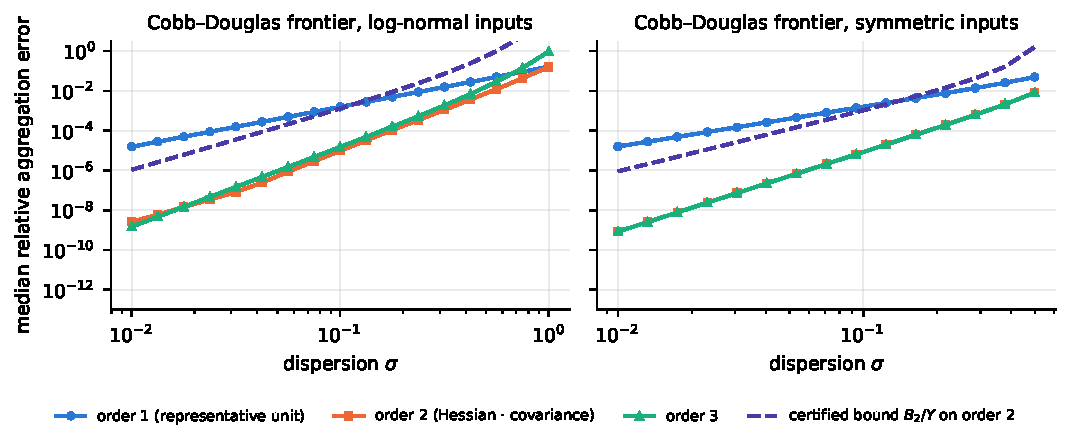
\includegraphics[width=0.9\linewidth]{../figures/dispersion_sweep.pdf}
\caption{E1, Cobb--Douglas frontier (the CES curves are the same up to constants; Table~\ref{tab:e1}). Median relative aggregation error against dispersion for the three orders and the certified bound $B_2/Y$ on the second-order error. Slopes $2$, $4$ ($3$--$4$ on skewed inputs at this $N$) and $4$.}
\label{fig:sweep}
\end{figure}

\emph{Criterion C1.} On symmetric inputs C1 holds on the whole sweep for both frontiers (minimum ratios $\EoneRtoAtMaxCDSU$ and $\EoneRtoAtMaxCESSU$ at $\sigma=\EoneSigmaMaxCDSU$). On log-normal inputs it holds at $\sigma=\EoneConeLargestCDLN$ and fails at the next grid point, $\sigma=\EoneConeFirstFailCDLN$ (both frontiers); at $\sigma=\EoneSigmaMaxCDLN$ the minimum ratio is $\EoneRtoAtMaxCDLN$ (CD) and $\EoneRtoAtMaxCESLN$ (CES), that is, the second-order approximation is then \emph{worse} than the representative unit.

\emph{Third order.} On log-normal inputs the median ratio $|E_2|/|E_3|$ is below $1$ in $\EoneRttCellsCDLN$ of $\EoneCellsCDLN$ cells for Cobb--Douglas and $\EoneRttCellsCESLN$ of $\EoneCellsCESLN$ for CES: adding the third moment does not improve the aggregate, as Remark~\ref{rem:orders} anticipates, and at large dispersion it degrades it substantially (minimum ratio $\EoneRttMinCDLN$). On symmetric inputs $\Yh_3=\Yh_2$ exactly.

\emph{Bounds and certificate.} The segmentwise bound $B_2$ holds in every replication and cell of both input laws (checks: \EoneBoundHoldsCDLN, \EoneBoundHoldsCDSU), as does the cruder single-box bound. It is conservative: the largest observed $|E_2|/B_2$ is $\EoneEtwoOverBtwoMaxCDLN$ (LN) and $\EoneEtwoOverBtwoMaxCDSU$ (SU), because the actual error cancels to order $\sigma^3$--$\sigma^4$ while the bound is built from the absolute third moment. The improvement is certifiable from moments alone when $2B_2<|Q_2|$ (Proposition~\ref{prop:smooth}(e)); this holds in every replication only for $\sigma\le\EoneCertSigmaCDLN$ (LN) and $\sigma\le\EoneCertSigmaCDSU$ (SU), whereas the improvement itself is observed up to $\sigma=\EoneConeLargestCDLN$. (The weaker comparison of the median bound with the median true first-order error, which is not observable from moments and omits the factor $2$, would extend to $\sigma\le\EoneBoundSigmaNonobsCDLN$ and $\EoneBoundSigmaNonobsCDSU$; it is not a certificate.)

\emph{Efficiency terms (E1b).} Same design (Cobb--Douglas, LN, $N=\EonebN$, \EonebReps{} replications) with independent efficiencies $\theta_i\sim U(0.5,1)$, $\mathrm{sd}(\theta)/\bar\theta=\EonebSdTheta$. The covariance term $C/Y^\theta$ of Remark~\ref{rem:eff} exceeds the second-order remainder up to $\sigma=\EonebSigmaCov$ and is $\EonebRatioSmallest$ times larger than it at $\sigma=0.01$; its median is $\EonebPredMin$--$\EonebPredMax$ of the predicted standard deviation $\mathrm{sd}(\theta)\mathrm{CV}_u/(\bar\theta\sqrt N)$ (the median of $|Z|$ for a standard normal $Z$ is $0.67$). With unobserved idiosyncratic efficiency the refinement from the first to the second order is below the sampling floor unless the input dispersion is large or the population is very large.

\subsection{E2: capacity thresholds}

Cobb--Douglas frontier, $N=\EtwoN$, $\EtwoReps$ replications, both input laws, capacity $c=f(\bar x)/(1+\delta)$ with $\delta\in\{\EtwoDeltas\}$ (negative: the representative unit is below capacity) and $\sigma$ from $\EtwoSigmaMin$ to $1$ ($0.5$ for SU). Figure~\ref{fig:threshold} (top) and Table~\ref{tab:e2}; the full grid is in \texttt{results/tables.md}.

\begin{table}[t]
\centering\footnotesize\setlength{\tabcolsep}{3.5pt}
\begin{tabular}{lrrrrrrrrrr}
\toprule
law & $\sigma$ & $|e_1|$ & $|e_2|$ & $|e_2|$ (smooth) & $\min\frac{|E_1|}{|E_2|}$ & below branch & above (\%) & $\frac{-E_2}{N\Tu}$ & $\frac{\Tu}{\sigma\tau_z}$ & $\frac{\Tu}{\sigma\tau_z(b)}$\\
\midrule
-0.30 & 0.01 & \ensuremath{1.5\times 10^{-5}} & \ensuremath{3.7\times 10^{-9}} & \ensuremath{3.7\times 10^{-9}} & 2101.28 & \ensuremath{0} & -- & 0.00 \\
-0.30 & 0.0316 & \ensuremath{1.5\times 10^{-4}} & \ensuremath{1.5\times 10^{-7}} & \ensuremath{1.5\times 10^{-7}} & 493.85 & \ensuremath{0} & -- & 0.00 \\
-0.30 & 0.1 & \ensuremath{1.6\times 10^{-3}} & \ensuremath{1.2\times 10^{-5}} & \ensuremath{1.2\times 10^{-5}} & 85.64 & \ensuremath{0} & -- & 0.00 \\
-0.30 & 0.316 & \ensuremath{2.1\times 10^{-2}} & \ensuremath{4.1\times 10^{-3}} & \ensuremath{1.2\times 10^{-3}} & 4.20 & \ensuremath{5.3\times 10^{-3}} & 0.773 & 0.04 \\
-0.03 & 0.01 & \ensuremath{1.6\times 10^{-5}} & \ensuremath{3.7\times 10^{-9}} & \ensuremath{3.7\times 10^{-9}} & 18.69 & \ensuremath{0} & 0.999 & 0.00 \\
-0.03 & 0.0316 & \ensuremath{1.0\times 10^{-3}} & \ensuremath{8.5\times 10^{-4}} & \ensuremath{1.5\times 10^{-7}} & 1.15 & \ensuremath{8.5\times 10^{-4}} & 1.000 & 0.08 \\
-0.03 & 0.1 & \ensuremath{1.7\times 10^{-2}} & \ensuremath{1.5\times 10^{-2}} & \ensuremath{1.2\times 10^{-5}} & 1.10 & \ensuremath{1.5\times 10^{-2}} & 0.999 & 0.31 \\
-0.03 & 0.316 & \ensuremath{9.0\times 10^{-2}} & \ensuremath{7.2\times 10^{-2}} & \ensuremath{1.2\times 10^{-3}} & 1.23 & \ensuremath{7.3\times 10^{-2}} & 0.983 & 0.37 \\
+0.00 & 0.01 & \ensuremath{2.8\times 10^{-3}} & \ensuremath{2.8\times 10^{-3}} & \ensuremath{3.7\times 10^{-9}} & 1.00 & \ensuremath{2.7\times 10^{-3}} & 1.000 & 0.50 \\
+0.00 & 0.0316 & \ensuremath{8.8\times 10^{-3}} & \ensuremath{8.7\times 10^{-3}} & \ensuremath{1.5\times 10^{-7}} & 1.00 & \ensuremath{8.7\times 10^{-3}} & 1.000 & 0.49 \\
+0.00 & 0.1 & \ensuremath{2.9\times 10^{-2}} & \ensuremath{2.8\times 10^{-2}} & \ensuremath{1.2\times 10^{-5}} & 1.00 & \ensuremath{2.8\times 10^{-2}} & 1.000 & 0.48 \\
+0.00 & 0.316 & \ensuremath{1.0\times 10^{-1}} & \ensuremath{9.4\times 10^{-2}} & \ensuremath{1.2\times 10^{-3}} & 1.00 & \ensuremath{8.8\times 10^{-2}} & 1.056 & 0.43 \\
+0.10 & 0.01 & \ensuremath{2.0\times 10^{-16}} & \ensuremath{2.0\times 10^{-16}} & \ensuremath{3.7\times 10^{-9}} & 1.00 & \ensuremath{0} & -- & 1.00 \\
+0.10 & 0.0316 & \ensuremath{2.0\times 10^{-16}} & \ensuremath{2.0\times 10^{-16}} & \ensuremath{1.5\times 10^{-7}} & 1.00 & \ensuremath{0} & -- & 1.00 \\
+0.10 & 0.1 & \ensuremath{3.0\times 10^{-3}} & \ensuremath{3.0\times 10^{-3}} & \ensuremath{1.2\times 10^{-5}} & 1.00 & \ensuremath{3.0\times 10^{-3}} & 1.000 & 0.90 \\
+0.10 & 0.316 & \ensuremath{6.0\times 10^{-2}} & \ensuremath{6.0\times 10^{-2}} & \ensuremath{1.2\times 10^{-3}} & 1.00 & \ensuremath{6.0\times 10^{-2}} & 1.000 & 0.60
\\
\bottomrule
\end{tabular}
\caption{E2 at $\delta=0$ (mean output on the capacity). ``Smooth'' is the error of the same population on the uncapped frontier; the improvement ratio is the minimum over all replications and over the replications whose sample mean falls below the capacity (``below branch''); ``above'' is the percentage of replications whose sample mean falls above it (SU: fixed to the below branch by convention); the last three columns are medians of the ratios of Proposition~\ref{prop:cap} and Corollary~\ref{cor:cross}, with $\tau_z(b)$ the shifted version of Remark~\ref{rem:hyp}(i).}
\label{tab:e2}
\end{table}

\begin{figure}[t]
\centering
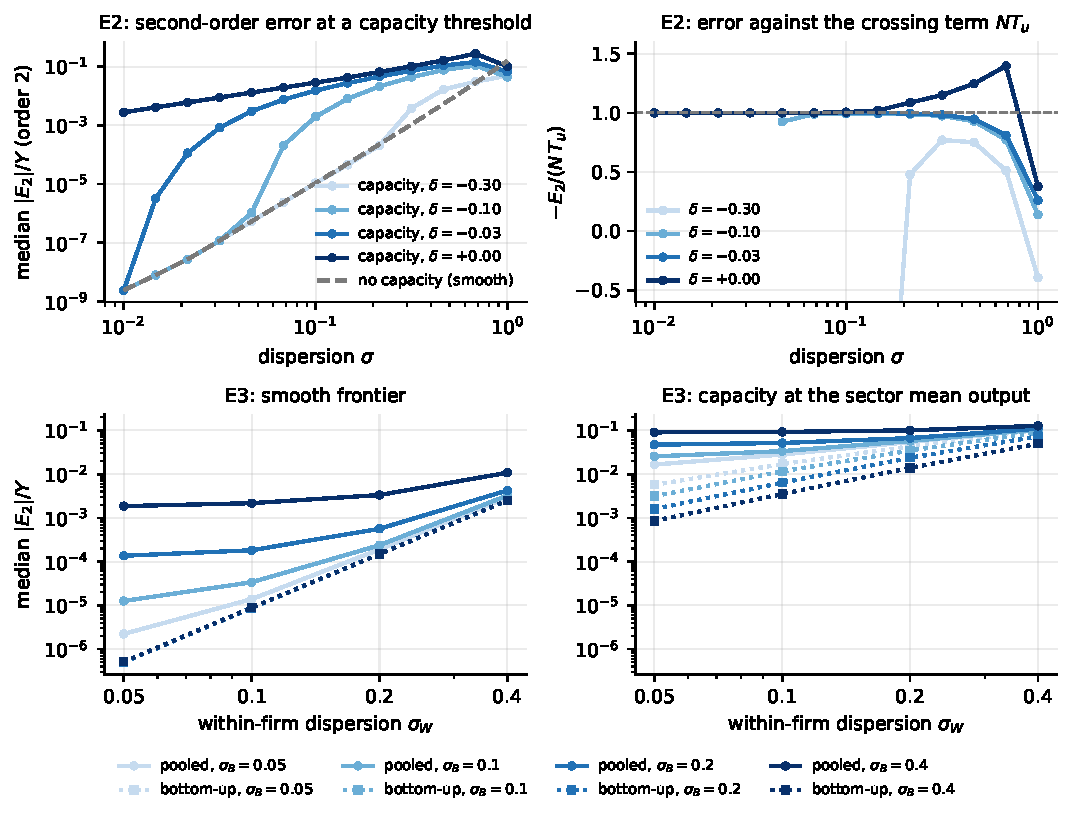
\includegraphics[width=0.84\linewidth]{../figures/threshold_hierarchy.pdf}
\caption{Top (E2, log-normal inputs): second-order relative error against dispersion for the capped frontier at four threshold proximities and for the uncapped frontier (left); the ratio $-E_2/(N\Tu)$, equal to $1+O(\sigma)$ by Proposition~\ref{prop:cap} (right; one point of $\delta=-0.30$ at $\sigma\approx\EtwoRatioClippedSigma$, where $N\Tu$ is smaller than the smooth error and the ratio is $\EtwoRatioClipped$, lies below the axis). Bottom (E3): pooled (solid) and bottom-up (dotted) second-order errors against within-firm dispersion, one shade per between-firm dispersion, for the smooth frontier (left) and with a capacity at the sector mean output (right).}
\label{fig:threshold}
\end{figure}

With the mean on the capacity ($\delta=0$) the small-dispersion exponent of the second-order error is $\EtwoSlopeCappedLN$ (LN) and $\EtwoSlopeCappedSU$ (SU), against $\EtwoSlopeSmoothLN$ and $\EtwoSlopeSmoothSU$ for the same populations on the uncapped frontier: the error is linear in the dispersion, as Corollary~\ref{cor:cross} states. At $\sigma=\EtwoSigmaMin$ the capped error is $\EtwoEtwoCapped$ (bootstrap interval $[\EtwoEtwoCappedLo,\EtwoEtwoCappedHi]$) against $\EtwoEtwoSmooth$ uncapped, an amplification of $\EtwoAmplification$. The constant of the corollary is checked on the symmetric design, to which it applies verbatim: the median of $\Tu/(\sigma\tau_z)$ is $\EtwoTauSU$ at $\sigma=\EtwoSigmaMin$ (bootstrap interval $\EtwoTauSUci$), $\EtwoTauSUPointOne$ at $\sigma=0.1$ and $\EtwoTauSUPointThree$ at $\sigma=0.316$, a deviation linear in $\sigma$ as the corollary's bound says. On the log-normal design the sample mean is not on the capacity ($|f(\bar x)-c|/c$ up to $\EtwoFxbarMinusCSmallLN$ at $\sigma=0.01$ and $\EtwoFxbarMinusCPointThreeLN$ at $\sigma=0.316$), so the unshifted ratio is $\EtwoTauLN$ at $\sigma=0.01$ while the shifted ratio $\Tu/(\sigma\tau_z(b))$ of Remark~\ref{rem:hyp}(i) is $\EtwoTaubLN$, then $\EtwoTaubLNPointOne$ and $\EtwoTaubLNPointThree$ at $\sigma=0.1$ and $0.316$. Identity \eqref{eq:capid} holds to a relative $\EtwoIdentityGap$ in all $\EtwoCells$ cells (a check of the code, not of the theory), so the ratio $-E_2/(N\Tu)$ of Table~\ref{tab:e2} is not an independent test of the constant: in the below branch it equals $1-E_2(f)/(N\Tu)$, and in the above branch with $\bar u>c$ it equals $1$ exactly. Likewise the two-sided bound \eqref{eq:capbound} holds in \EtwoTwoSided{} cells because it reduces to $B_1\ge|E_1(f)|$ and $B_2\ge|E_2(f)|$, already checked in E1; its lower-bound form $|E_2(f_c)|\ge N\Tu-B_1-B_2-|Q_2|\mathbf 1\{\cdot\}$ is informative exactly when $N\Tu$ exceeds the smooth bounds, which at $\delta=0$ (LN) happens for $\sigma\le\EtwoLowerSigmaLN$ and in $\EtwoLowerInformative$ of the $\EtwoCells$ cells overall; outside that range \eqref{eq:capid} remains an exact identity.

At $\delta=0$ the sample mean lies on either side of the capacity: by sampling for LN (above in $\EtwoFracAboveLNmin$--$\EtwoFracAboveLNmax\%$ of the replications along the sweep), and by floating-point rounding for SU, which we fix to the below branch (an explicit argument of the code with a relative tolerance of $10^{-12}$; the opposite convention puts $\EtwoFracAboveSUaltMin\%$ of the SU replications in the above branch). In the above branch $\Yh_2=\Yh_1$ by construction, so the minimum improvement ratio over all replications is exactly $1$ by definition ($\EtwoRtoAltSU$ for SU under the opposite convention); the informative figure is the below-branch ratio, $\EtwoRtoBelowLN$ (LN) and $\EtwoRtoBelowSU$ (SU) at $\sigma=\EtwoSigmaMin$, which grows slowly with $\sigma$ (Table~\ref{tab:e2}): the second order buys nothing at a crossing, in either branch. Away from the capacity ($\delta=-0.3$) the small-dispersion behaviour is that of the smooth frontier (minimum improvement ratio $\EtwoRtoFarSmall$ for $\sigma\le0.05$) until the upper tail of the population reaches the capacity, after which the error switches to the crossing regime; at $\delta=-0.03$ the switch occurs inside the fitting window and produces the transitional slope $\EtwoSlopeTransition$ visible in Figure~\ref{fig:threshold}. Units lie on both sides of the capacity in $\EtwoCrossingCells$ of the $\EtwoCells$ cells.

\subsection{E3: two-level hierarchy}

$G=\EthreeG$ firms of $n=\Ethreen$ units ($N=\EthreeN$), firm means log-normal around the sector mean with between-firm dispersion $\sigma_B$, units log-normal around their firm mean with within-firm dispersion $\sigma_W$, both in $\{0.05,0.1,0.2,0.4\}$, $\EthreeReps$ replications; smooth Cobb--Douglas frontier and the same frontier capped at the sector mean output. Figure~\ref{fig:threshold} (bottom); the table of all cells, with bootstrap intervals, is in \texttt{results/tables.md}. The identity $\Yh_2^{\mathrm{TD}}=\Yh_2$ of Lemma~\ref{lem:hier}(i) holds to a relative $\EthreeLemmaGap$ (floating point). On the smooth frontier the bottom-up estimator is better in $\EthreeBetterCells$ of $\EthreeCells$ cells, by a median per-replication factor from $\EthreeGainMin$ (small $\sigma_B$, large $\sigma_W$; median errors $\EthreePooledTwoLowBHighW$ and $\EthreeHierTwoLowBHighW$) to $\EthreeGainMax$ (large $\sigma_B$, small $\sigma_W$; median errors $\EthreePooledTwoHighBLowW$, interval $[\EthreePooledTwoHighBLowWLo,\EthreePooledTwoHighBLowWHi]$, and $\EthreeHierTwoHighBLowW$, interval $[\EthreeHierTwoHighBLowWLo,\EthreeHierTwoHighBLowWHi]$); the bottom-up error depends on $\sigma_W$ only, as Lemma~\ref{lem:hier}(ii) says, and the bound checks of Lemma~\ref{lem:hier}(ii) and Proposition~\ref{prop:smooth}(c) pass in every replication (all hold: \EthreeBoundsHold). With the capacity, $\EthreeStraddleMin$--$\EthreeStraddleMax\%$ of the firms straddle it; the bottom-up error is $\EthreeCappedRatioMin$--$\EthreeCappedRatioMax$ times the pooled one, and the firms that do not straddle contribute at most a fraction $\EthreeNonStraddleShare$ of the bottom-up error: the hierarchy localises the failure but does not remove it, since inside a straddling firm Corollary~\ref{cor:cross} applies.

\subsection{E4: rank reversals between two sectors}

Two sectors of $N=\EfourN$ units each. Sector $A$ has mean $\bar x$ and dispersion $\sigma$; sector $B$ has mean $\bar x(1+\gamma)^{1/0.8}$, so that $f(\bar x_B)=(1+\gamma)f(\bar x_A)$ with $\gamma$ uniform on $\pm\EfourGammaMax\%$, and dispersion $\sigma/2$. Inputs log-normal; $\EfourTrials$ trials per cell; $\sigma\in\{\EfourSigmaMin,\dots,\EfourSigmaMax\}$; capacity at $+50,+20,+10,+5,+0\%$ of $f(\bar x_A)$ or absent. A trial is a reversal at order $k$ when $\operatorname{sign}(\Yh_k^A-\Yh_k^B)\ne\operatorname{sign}(Y^A-Y^B)$. In the smooth cells a comparison is \emph{certified} when the margin condition of Proposition~\ref{prop:margin} holds with the bounds $B_2$ of the two samples. Table~\ref{tab:e4} (with Wilson 95\% intervals) and Figure~\ref{fig:decision}.

\begin{table}[t]
\centering\scriptsize\setlength{\tabcolsep}{2.5pt}
\begin{tabular}{rlllrrll}
\toprule
& \multicolumn{5}{c}{no capacity} & \multicolumn{2}{c}{capacity $+0\%$}\\
\cmidrule(lr){2-6}\cmidrule(lr){7-8}
$\sigma$ & rev.~1 & rev.~2 & rev.~3 & certified & cert.\ rev. & rev.~1 & rev.~2\\
\midrule
0.02 & 0.1 & 0.0 & 0.0 & 100 & 0 & 0.1 & 0.0 & 28.2 & 28.1 & 28.1 \\
0.05 & 0.3 & 0.0 & 0.0 & 100 & 0 & 0.3 & 0.0 & 35.5 & 35.3 & 35.3 \\
0.1 & 1.0 & 0.0 & 0.2 & 97 & 0 & 4.6 & 3.6 & 47.3 & 46.8 & 46.9 \\
0.2 & 4.0 & 0.3 & 0.1 & 71 & 0 & 22.7 & 18.4 & 67.5 & 65.3 & 65.3 \\
0.4 & 17.5 & 3.3 & 5.0 & 0 & 0 & 49.9 & 29.1 & 70.1 & 60.5 & 63.8 \\
0.8 & 45.2 & 2.8 & 89.2 & 0 & 0 & 48.1 & 0.1 & 62.0 & 48.8 & 93.8
\\
\bottomrule
\end{tabular}
\caption{E4. Rank-reversal rates in percent at orders $1$--$3$ over \EfourTrials{} trials per cell, with Wilson 95\% intervals for the rates that enter C2 (order 3 with the capacity is in Figure~\ref{fig:decision}); ``certified'' is the percentage of trials satisfying the margin condition with second-order bounds and ``cert.\ rev.'' the number of reversals among them. The other capacity positions are in Figure~\ref{fig:decision} and \texttt{results/tables.md}.}
\label{tab:e4}
\end{table}

\begin{figure}[t]
\centering
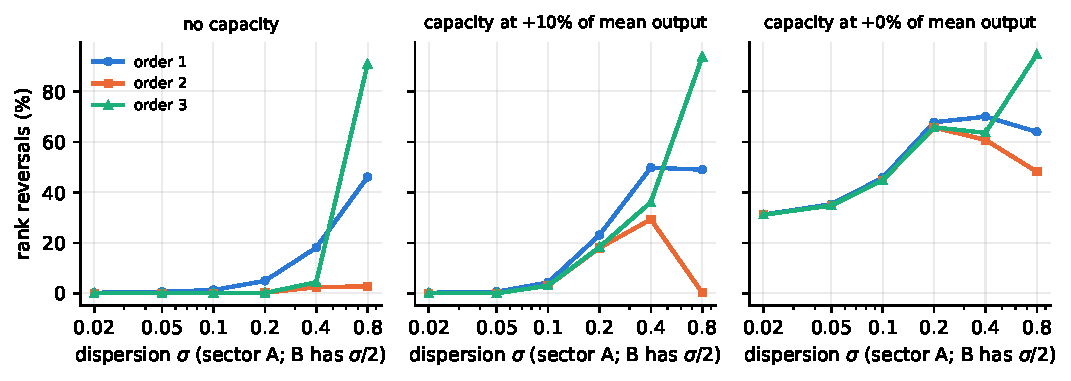
\includegraphics[width=0.9\linewidth]{../figures/decision.pdf}
\caption{E4. Rank-reversal rates against the dispersion of sector $A$ without capacity and with the capacity at $+10\%$ and $+0\%$ of its mean output.}
\label{fig:decision}
\end{figure}

Without capacity the second order removes almost all reversals: the first-order rate reaches $\EfourSmoothRevOneMax\%$ and the second-order rate never exceeds $\EfourSmoothRevTwoMax\%$. Among the certified comparisons there were $\EfourCertifiedReversals$ reversals at order~2 (and $\EfourCertifiedOneReversals$ among comparisons certified with first-order bounds), as Proposition~\ref{prop:margin} requires; but the certificate covers $\EfourCertFracSmall\%$ of the trials at $\sigma=\EfourSigmaMin$, $\EfourCertFracPointTwo\%$ at $\sigma=0.2$ and $\EfourCertFracPointFour\%$ at $\sigma=0.4$. The third order is harmful at large dispersion: at $\sigma=\EfourSigmaMax$ its reversal rate is $\EfourRevThreeLargeSigma\%$, against $\EfourRevOneLargeSigma\%$ for the first and $\EfourRevTwoLargeSigma\%$ for the second order, because the third central moments of log-normal inputs over-correct. With the capacity at the mean output of $A$ the reversal rates are $\EfourCapZeroRevOneSmall\%$ (order~1) and $\EfourCapZeroRevTwoSmall\%$ (order~2) already at $\sigma=\EfourSigmaMin$, and the second-order rate stays between $\EfourCapRevTwoMin\%$ and $\EfourCapRevTwoMax\%$; with the capacity at $+10\%$ the crossing regime is entered at $\sigma\approx0.1$ (rates $\EfourCapTenRevOnePointTwo\%$ and $\EfourCapTenRevTwoPointTwo\%$ at $\sigma=0.2$).

\emph{Criterion C2.} Of the $\EfourEligible$ cells with a first-order reversal rate of at least $2\%$ ($\EfourEligibleSmooth$ without capacity, $\EfourEligibleCapped$ with it), $\EfourFailing$ fail C2 on the point estimates, all with a capacity. Taking the Wilson intervals into account (a cell fails clearly when the lower limit of the second-order rate exceeds one fifth of the upper limit of the first-order rate, passes clearly in the mirror case, and is borderline otherwise), C2 fails clearly in $\EfourFailClearCapped$ capacity cells, is borderline in $\EfourBorderline$ cells (\EfourBorderlineCellsText; in the smooth one the rates are $\EfourSmoothRevOnePointFour\%$ $\EfourSmoothRevOnePointFourCi$ and $\EfourSmoothRevTwoPointFour\%$ $\EfourSmoothRevTwoPointFourCi$) and passes clearly in the remaining $\EfourPassClearSmooth$ smooth and $\EfourPassClearCapped$ capacity cells. The capacity cells that pass (\EfourPassingCellsText) are cells in which the sample mean of $A$ stays below the capacity in at least $\EfourPassingMeanBelowMin\%$ of the trials, so the approximations do not see the capacity and the second order is right for reasons unrelated to the crossing; this is also why the rows $+50$, $+20$ and $+10\%$ at $\sigma=\EfourSigmaMax$ are nearly identical. C2 does not hold.

\subsection{E5: a scalar recalibration}

The record of the research line mentions a calibration that failed its criterion; the original procedure is not documented, so we test the simplest one. The second-order term is rescaled, $\Yh_\lambda=\Yh_1+\lambda Q_2$, with $\lambda$ fitted by least squares on a training design (Cobb--Douglas, LN, $N=\EfiveN$, $\EfiveReps$ replications, $\sigma\in\{\EfiveTrainSigmas\}$, four regimes: no capacity, and $f(\bar x)/c-1\in\{-0.1,0,+0.1\}$), either globally or separately by regime, and evaluated on new seeds at off-grid dispersions $\sigma\in\{\EfiveTestSigmas\}$ for both input laws; the criterion is C1 on the test grid. The fitted values are $\lambda=\EfiveLambdaGlobal$ (global) and $\EfiveLambdaSmooth$, $\EfiveLambdaBelow$, $\EfiveLambdaAt$ for the smooth, below and at-capacity regimes; above capacity $Q_2\equiv0$, no $\lambda$ exists and there is nothing to recalibrate, so that regime is reported as not applicable and excluded from the verdict. Table~\ref{tab:e5}.

\begin{table}[t]
\centering\small
\begin{tabular}{llrrr}
\toprule
law & regime & order 2 ($\lambda=1$) & global $\lambda$ & regime $\lambda$\\
\midrule
LN & smooth & 2.22 & 0.44 & 3.39 \\
LN & below & 1.37 & 0.80 & 0.47 \\
LN & at (all replications) & 1.00 & 1.00 & 0.98 \\
LN & at (below branch only) & 1.02 & 1.04 & 0.98 \\
LN & above & n/a & n/a & n/a \\
SU & smooth & 19.18 & 0.80 & 6.50 \\
SU & below & 1.33 & 0.80 & 0.47 \\
SU & at (all replications) & 1.02 & 1.04 & 1.08 \\
SU & at (below branch only) & 1.02 & 1.04 & 1.08 \\
SU & above & n/a & n/a & n/a
\\
\bottomrule
\end{tabular}
\caption{E5. Minimum over the test dispersions and replications of $|E_1|/|Y-\Yh_\lambda|$; C1 requires at least $5$ everywhere. ``At'' is reported over all replications and over those whose sample mean falls below the capacity (LN: $\EfiveAtFracAboveLNMin$--$\EfiveAtFracAboveLNMax\%$ above; SU: below branch by convention); ``above'' is n/a because $Q_2\equiv0$. Per-dispersion values in \texttt{results/tables.md}.}
\label{tab:e5}
\end{table}

No variant meets C1 on the smooth, below and at-capacity regimes (order 2: \EfiveOtwoConeExclAbove; global: \EfiveGlobConeExclAbove; by regime: \EfiveRegConeExclAbove), and the substantive failures are in the smooth and below regimes. The global rescaling is worse than the representative unit in the smooth regime (minimum ratio $\EfiveGlobLNSmooth$), because a factor fitted to crossing cells destroys the $O(\sigma^3)$--$O(\sigma^4)$ accuracy where there is no crossing. The regime-specific factor helps at moderate dispersion below capacity but is worse than the representative unit at small dispersion (minimum ratio $\EfiveRegLNBelow$), where no unit crosses and the term it rescales should be left alone. At the capacity the below-branch ratios are $\EfiveOtwoLNAtBelow$, $\EfiveGlobLNAtBelow$ and $\EfiveRegLNAtBelow$ (LN): every variant is as good as the representative unit and no better, the mechanism of Example~\ref{ex:moments}: the error to be removed scales as $\sigma$, the only available regressor scales as $\sigma^2$, and no constant reconciles them across dispersions. The plain second order fails C1 on the test grid too (ratio $\EfiveOtwoLNSmooth$ at $\sigma=0.6$, consistent with E1).

\section{What can be claimed}\label{sec:claims}

\begin{table}[t]
\centering\scriptsize
\begin{tabular}{p{0.67\linewidth}p{0.27\linewidth}}
\toprule
claim & status\\
\midrule
First-order error is $N$ times the Jensen gap, non-positive for concave $f$ & classical\\
Remainder identities, bounds $B_1$, $B_2$, improvement ratio $\ge3\lambda/(M_3\rho)$, observable certificate (Prop.~\ref{prop:smooth}); bounds hold in every simulated population, $|E_2|/B_2\le\EoneEtwoOverBtwoMaxCDLN$, certificate up to $\sigma=\EoneCertSigmaCDLN$ (E1) & classical (Taylor), assembled here; verified\\
Exponents $2$ / $4$ / $4$ on symmetric inputs; $3$--$4$ for the second order on log-normal inputs at finite $N$ (Rem.~\ref{rem:orders}, E1, E1c) & consequence of Prop.~\ref{prop:smooth}; verified\\
Third order does not improve on the second for log-normal inputs (Rem.~\ref{rem:orders}, E1) & heuristic; verified\\
Top-down two-stage second order equals the pooled one (Lem.~\ref{lem:hier}(i)) & elementary (total covariance); by construction of Def.~\ref{def:hier}\\
Bottom-up error is the sum of within-firm errors; gain $\EthreeGainMin$--$\EthreeGainMax$ (Lem.~\ref{lem:hier}(ii), E3) & elementary; verified\\
Hinge identity (Lem.~\ref{lem:hinge}); $E_2(f_c)=-N\Tu+O(\text{smooth terms})$ (Prop.~\ref{prop:cap}); identity checked to $\EtwoIdentityGap$ (E2) & elementary / proved here; verified\\
At a crossing the error is $\Theta(\sigma)$, $|E_1|/|E_2|\to1$, $\Tu=\sigma\tau_z+O(\sigma^2)$ (Cor.~\ref{cor:cross}); slope $\EtwoSlopeCappedSU$, $\Tu/(\sigma\tau_z)=\EtwoTauSU$ at $\sigma=\EtwoSigmaMin$ (E2, SU) & proved here; verified\\
Populations with equal first three moments and aggregates differing at order $\sigma$ (Ex.~\ref{ex:moments}) & proved here\\
Margin condition preserves the ordering (Prop.~\ref{prop:margin}); $\EfourCertifiedReversals$ reversals among certified pairs; certificate for $\EfourCertFracPointFour\%$ of pairs at $\sigma=0.4$ (E4) & elementary; verified\\
Covariance floor $O(\sigma/\sqrt N)$ with independent efficiencies (Rem.~\ref{rem:eff}); dominates up to $\sigma=\EonebSigmaCov$ (E1b) & elementary; verified\\
Predefined C1 holds on the SU sweep; fails on the LN sweep beyond $\sigma=\EoneConeLargestCDLN$; fails at crossings. Predefined C2 fails clearly in $\EfourFailClearCapped$ of $\EfourEligibleCapped$ capacity cells, $\EfourBorderline$ cells borderline. A scalar recalibration of $Q_2$ does not meet C1 (E5) & verified\\
Statements about real sectors, estimated frontiers or policy & not addressed\\
\bottomrule
\end{tabular}
\caption{Claims and their status. ``Verified'' means reproduced by the script of Appendix~\ref{app:repro} with the fixed seed; it is not a proof. The original content of the draft is the combination Prop.~\ref{prop:cap}, Cor.~\ref{cor:cross}, Ex.~\ref{ex:moments} and the experiments.}
\label{tab:claims}
\end{table}

Table~\ref{tab:claims} is the deliverable of the research line: it separates what is classical from what is proved here and from what is measured, and it records that the predefined criterion of a general certified improvement was not met. The positive content is precise: in the smooth regime the second-order correction reduces the error by a factor of order $\sigma$ and comes with a computable certificate that is very conservative (valid for $\sigma\lesssim\EoneCertSigmaCDLN$); at a capacity crossing it is no improvement at all, the missing quantity $\Tu$ is not a function of the moments, and no rescaling of the moment term supplies it.

\paragraph{Limitations.} The frontier is known exactly; estimation error in $f$ or in the moments is not modelled, and would add to every error reported. The certified bounds are computed only for Cobb--Douglas, where the derivative suprema have closed forms; for CES a bound would need a numerical supremum, which we did not certify. The bounds are loose by a factor of about $50$--$1000$ at moderate dispersion because they use absolute third moments where the actual error cancels. Two input laws and two frontiers are a controlled design, not a survey of shapes; the crossing analysis covers the capacity kink $\min(f,c)$ and, by the same proof, any frontier with a first-derivative jump along a hypersurface, but not regime switches that also change the level. The hierarchy has two levels; deeper hierarchies compose Lemma~\ref{lem:hier}. The decision experiment uses one margin distribution ($\pm\EfourGammaMax\%$), one dispersion ratio between sectors and $\EfourTrials$ trials per cell, which leaves $\EfourBorderline$ of its $\EfourEligible$ eligible cells undecided.

\paragraph{Next steps.} (a) A sharper certificate that exploits cancellation, for instance a bound of $E_2$ by the third central moment tensor plus a fourth-order remainder, which would extend the certified region beyond $\sigma\approx\EoneCertSigmaCDLN$. (b) The crossing term $\Tu$ is the Jensen gap of the hinge; estimating it from a parametric family fitted to $(\bar x,\Sigma)$ is exact within the family and should be tested out of family, with Example~\ref{ex:moments} as the worst case. (c) Efficiency terms correlated with inputs, where $C$ acquires a mean that the moment expansion must model. (d) The dynamic element the line's name promises: a trajectory $\sigma_t$ or $\bar x_t$ approaching the capacity, for which Proposition~\ref{prop:cap} and Remark~\ref{rem:hyp}(i) already give $E_2(t)$ and the regime switch. (e) Any statement about a real sector needs an estimated frontier and its sampling error first; nothing here licenses that step.

\appendix
\section{Reproducibility}\label{app:repro}
{\sloppy The directory contains \path{experiments/frontier_aggregation.py} (E0--E6, flag \texttt{--fast} for a reduced run; one random generator per experiment spawned from the master seed) and \path{experiments/make_numbers.py}, which converts \path{results/results.json} into the macros and table bodies used by this document, so that every number in the text is generated and none is typed. The reference run used seed \MetaSeed, Python \MetaPython, NumPy \MetaNumpy{} \citep{harris2020} and SciPy \MetaScipy{} \citep{virtanen2020}; it took \MetaSeconds{} seconds of wall time (\MetaCpuSeconds{} s of CPU) on shared cores, and its script hash is \MetaScriptSha. The closed-form gradient, Hessian and third-derivative tensor of both frontiers are implemented in the classes \texttt{CobbDouglas} and \texttt{CES} and checked by E0 against central differences. Bounds: for each unit the coordinate box spanned by $\bar x$ and $x_i$; each entry of $D^2\!f$, $D^3\!f$ bounded at the corner given by the sign of its exponent; Frobenius norm of the entrywise bounds; $B_1=\frac12\sum M_2^{(i)}\|h_i\|^2$, $B_2=\frac16\sum M_3^{(i)}\|h_i\|^3$. Input laws: standard shocks $z$ with correlation $\EoneCorr$ (Cholesky); LN $x=\bar x\odot\exp(\sigma z-\sigma^2/2)$; SU $w=\sqrt3(2\Phi(z)-1)$ on half the sample and $-w$ on the other half, $x=\bar x\odot(1+\sigma w)$. E3: firm means $\bar x\odot\exp(\sigma_B\zeta-\sigma_B^2/2)$, units $\bar x_g\odot\exp(\sigma_Wz-\sigma_W^2/2)$, capacity $c=f(\bar x)$. E4: $\gamma\sim U(-0.05,0.05)$, $\bar x_B=\bar x_A(1+\gamma)^{1/0.8}$, $\sigma_B=\sigma_A/2$, capacity $c=f(\bar x_A)(1+p)$, certification with $|\Yh_2^A-\Yh_2^B|>B_2^A+B_2^B$, Wilson intervals with $z=1.96$. E5: $\lambda=\sum E_1Q_2/\sum Q_2^2$ over the training cells, globally or within each regime; evaluation on fresh shocks. Uncertainty: percentile bootstrap over replications ($1000$ resamples) for medians, and over replications with refitting ($500$ resamples) for exponents.\par}

\providecommand{\bibfont}{}\renewcommand{\bibfont}{\footnotesize}
\bibliographystyle{plainnat}
\bibliography{refs}
\end{document}
